\section{PHY Layer}
\label{sec:phy}

\subsection{Numerology}

The waveform is designed to pass through an ordinary SSB transceiver's
audio path (AGC off).  Table~\ref{tab:numerology} lists the parameters,
all taken from the article~\cite{habr_ofdm}.

\begin{table}[H]
    \centering
    \caption{OFDM numerology.}
    \label{tab:numerology}
    \small
    \begin{tabular}{@{}lp{8.5cm}@{}}
    \toprule
    \textbf{Parameter} & \textbf{Value} \\
    \midrule
    Sample rate       & 12\,kHz \\
    FFT size          & 128 bins $\rightarrow$ 93.75\,Hz subcarrier spacing \\
    Occupied band     & 300--2400\,Hz $\rightarrow$ bins 3--25, 23 subcarriers \\
    Pilots            & 7, Zadoff--Chu root 3, bins 3, 6, 10, 14, 17, 21, 25 \\
    Data carriers     & 16 \\
    Cyclic prefix     & 32 samples (25\,\%) \\
    Symbol tiling     & $4\times$ / $16\times$ / $64\times$ by link mode
                        (+6\,dB per $4\times$, coherent) \\
    CFO tolerance     & $\pm$375\,Hz design, $\pm$300\,Hz specified \\
    \bottomrule
    \end{tabular}
\end{table}

Two consequences of that grid are worth stating explicitly, because
everything downstream is measured against them.

\emph{One symbol carries 16 modulation symbols.}  With 16 of the 23
subcarriers carrying data, a single OFDM symbol holds $16\mu$ coded
bits before tiling --- 16 at BPSK, 32 at QPSK, 64 at 16-QAM --- and the
tiling factor then divides the rate by 4, 16 or 64.  The whole ladder
of Section~\ref{sec:modes}, from 7.8 to 1059\,bit/s, is that one
number multiplied by a modulation order, a code rate and a tiling
factor; nothing else in the waveform moves.

\emph{Seven of twenty-three carriers are pilots.}  Roughly 30\,\% of
the grid is spent on channel estimation, every symbol, at every rung.
That is a deliberate choice for HF: pilots every 3--4 bins track a
fading channel across the 2.1\,kHz occupied band, and the Wiener
estimator built on them is what makes coherent accumulation over 64
tiled repeats possible at all.  It is also the single largest rate
saving still available --- reclaiming even half of it would beat every
coding improvement measured in this report --- which is why pilot
reduction and 2-D channel estimation head the future-work list
(Section~\ref{sec:discussion}).  The pilot pattern is fixed by the
article and was not varied here; changing it would invalidate the
bit-exact reproduction that Section~\ref{sec:results} rests on.

Symbol \emph{tiling} is the article's central trick for negative-SNR
operation: each OFDM symbol body is repeated back-to-back
\texttt{sym\_tile} times, and the receiver accumulates the repeats
coherently before the FFT.  Each $4\times$ factor buys $\approx$6\,dB
of effective SNR at a $4\times$ rate cost.

\subsection{Frame Structure}

Every frame (Figure~\ref{fig:frame_structure}) carries a two-stage
preamble --- Newman-phased tone combs~\cite{newman1965} for detection
and coarse CFO, then Zadoff--Chu symbols for sample-exact timing ---
followed by a header and the data block.  The header (25 bits:
\texttt{ver(2)\,|\,typ(3)\,|\,mod(2)\,|\,spd(2)\,|\,len(8)\,|\,CRC-8})
is always sent in the most robust configuration (BPSK, rate-1/3, six
tiled symbols = 93 coded bits); its \texttt{mod}/\texttt{spd}/%
\texttt{len} fields drive the data-block demodulation, and
\texttt{ver=2} marks an LDPC-coded data block.  The CRC-8 is seeded
with $\mathrm{0xFF} \oplus \mathit{key}$, the link's \emph{net key}
(\S\ref{sec:net_key}); key 0 is the article's CRC
(Section~\ref{sec:coding}).  Preamble bins carry deliberate gain
($\times 2$ for ZC symbols, $\times\sqrt{5.75}$ for tone combs) so the
whole frame has uniform per-sample power --- Section~\ref{sec:sync}
shows why detection sensitivity depends on this.

\begin{figure}[H]
    \centering
    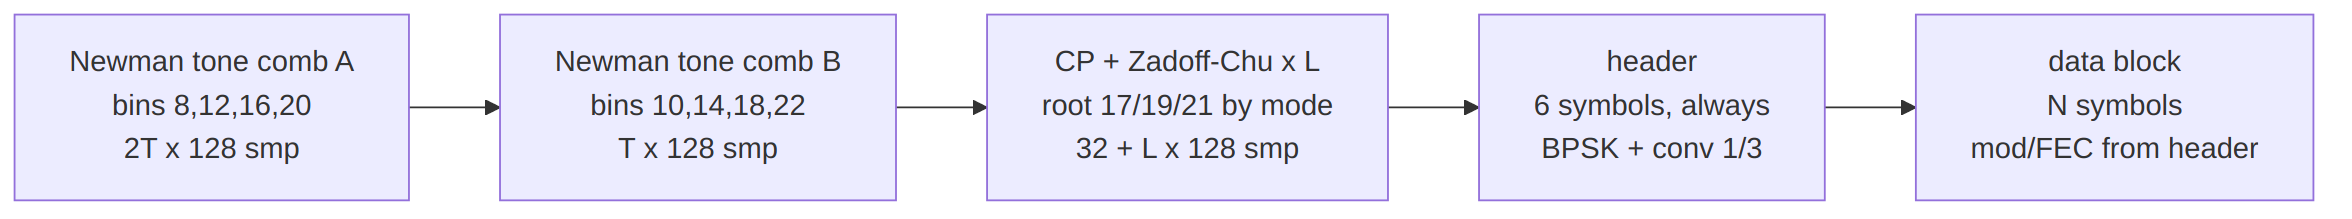
\includegraphics[width=\textwidth]{images/frame_structure.png}
    \caption{Frame structure.  $T$ is the mode's tone-tiling factor and
             $L$ the mode's Zadoff--Chu symbol count.}
    \label{fig:frame_structure}
\end{figure}

\subsection{The Zadoff--Chu Sequences: Definition and Computation}
\label{sec:zc}

Two of the three things a receiver locks onto are Zadoff--Chu
sequences~\cite{chu1972}: the seven pilots that carry the channel
estimate, and the preamble symbol that gives sample-exact timing and
names the link mode.  This subsection states the sequence exactly as
the code defines it, where each instance is placed, which of its
properties the receiver depends on, and how each of the three
implementations obtains it.

\paragraph{Definition.}  One generator serves both uses
(\texttt{OFDMModem.\_gen\_zc\_seq(root, length)}):
\begin{equation}
    z_u[n] \;=\; \exp\!\left(-\,j\pi\,\frac{u\,n\,(n + N \bmod 2)}{N}\right),
    \qquad n = 0, \ldots, N-1,
    \label{eq:zc}
\end{equation}
which is the standard Zadoff--Chu sequence of root $u$ and length $N$
with the cyclic-shift term $q = 0$: the factor $N \bmod 2$ selects
$n(n+1)$ for odd $N$ and $n^2$ for even $N$.  Both lengths used here
are odd, so both instances are of the $n(n+1)$ form.  The code computes
Eq.~\eqref{eq:zc} directly in double precision and casts the result to
\texttt{complex64}; nothing is tabulated in the float model.

\paragraph{Where the two instances are placed.}
Table~\ref{tab:zc_instances} lists both.  The pilot sequence is placed
one value per pilot carrier, in carrier order; the pilot carriers are
the seven equally spaced positions \texttt{linspace(0, 22, 7)} over
the 23 loaded bins, i.e.\ bins 3, 6, 10, 14, 17, 21 and 25.  The
preamble sequence fills the 23 loaded bins contiguously (bin
$14 - \lfloor 23/2 \rfloor = 3$ upward), with no Hermitian mirror and
a $\times 2$ gain that equalizes the real-signal power of a 23-bin
symbol against the 46 bins of a mirrored data symbol
(Section~\ref{sec:sync}).  A 128-point IFFT of that bin vector is one
ZC symbol; it is tiled $L$ times back to back and the block is closed
with a cyclic prefix that is the last 32 samples of the tiled block ---
so the CP is the tail of the last tile, and the block is periodic in
128 samples throughout.  The CP-plus-one-tile of 160 samples is also
what a streamed burst re-emits as its resync marker
(\S\ref{sec:stream}).

\begin{table}[H]
    \centering
    \caption{The two Zadoff--Chu instances, as instantiated.}
    \label{tab:zc_instances}
    \small
    \begin{tabular}{@{}lll@{}}
    \toprule
    & \textbf{Pilots} & \textbf{Preamble} \\
    \midrule
    length $N$ & 7 & 23 \\
    root $u$ & 3 & 17 / 19 / 21 (NORMAL / ROBUST / EXTREME) \\
    domain & one value per pilot carrier & one value per loaded bin, 3..25 \\
    gain & 1 (unit modulus) & $\times 2$ \\
    time structure & inside every data and header symbol &
        IFFT, tiled $L = 4 / 16 / 64$, CP $=$ last 32 samples \\
    receiver use & channel estimate at 7 carriers &
        timing, residual-CFO hypothesis, mode identity \\
    \bottomrule
    \end{tabular}
\end{table}

\paragraph{The properties the receiver relies on.}  Three, each
checked by the article-reproduction suite
(\texttt{verify\_article.py}, Appendix~\ref{app:verify}) or by
construction:
\begin{itemize}
    \item \textbf{Constant amplitude.}  $|z_u[n]| = 1$ for every $n$,
          so the zero-forcing estimate at a pilot carrier is
          $\hat H_k = Y_k\,\overline{p_k}$ --- a multiplication by the
          conjugate, no division.  The fixed-point and C receivers are
          division-free in channel estimation for exactly this reason
          (Section~\ref{sec:fixed}): the conjugate pilots are a Q15
          ROM, and the pilot-to-carrier interpolation is a second ROM
          of Wiener weights.
    \item \textbf{Zero periodic autocorrelation.}  For $N$ prime and
          $\gcd(u, N) = 1$ the periodic autocorrelation of $z_u$ is a
          delta: $\sum_n z_u[n]\,\overline{z_u[n-k]} = N$ at $k = 0$ and
          $0$ for every other shift (measured: $23, 0, \ldots, 0$ for
          the root-17 sequence).  This is what makes the matched-filter
          peak sharp to one sample, and the suite asserts it.
    \item \textbf{Distinct roots are near-orthogonal.}  With $N = 23$
          prime, every root in $1..22$ is admissible, and the
          cross-correlation of two different roots is $1/\sqrt{23}$ in
          magnitude at every lag.  The three modes use three roots, and
          the receiver identifies the mode by which root correlates
          (\texttt{demod\_frame\_auto} tries the modes in turn on the
          same samples, Section~\ref{sec:modes}); a mode switch can
          therefore never leave the two ends unable to find each other.
\end{itemize}

\paragraph{How the detector computes with it.}  The float detector
(\texttt{detect\_zc\_preamble}) builds its kernel from the
time-domain preamble block, not from Eq.~\eqref{eq:zc}: the kernel is
the last $G$ tiles of the generated block ($G$ the mode's coherent
group, $1 / 2 / 4$), so it carries the $\times 2$ gain and the IFFT
scaling exactly as transmitted.  For each residual-CFO hypothesis the
kernel is derotated, the signal is correlated with its reversed
conjugate by FFT convolution, the magnitudes of the $L/G$ group
positions are summed, and the sum is normalized by
$\sqrt{E_{\mathrm{win}}\,E_{\mathrm{ref}}}$ --- the energy of the
signal window against the kernel's own --- so the metric is a
correlation coefficient in $[0, 1]$ and a loud data symbol cannot
outscore the preamble.  The NORMAL detector evaluates one hypothesis
(zero: Section~\ref{sec:sync} explains why widening it costs a
decibel); ROBUST and EXTREME evaluate seven, $\pm 15$\,Hz in 5\,Hz
steps, because their longer coherent kernels tolerate less residual
offset.

\paragraph{How each twin obtains the sequence.}  The float model
computes it.  The fixed-point twin never does: it takes the float
model's pilot values and preamble block and rounds them to Q15
(\texttt{round}$(x \cdot 32767)$) into three ROMs --- the conjugate
pilots for estimation, the real part of the whole preamble for the
transmitter, and the complex $G \cdot 128$-sample kernel for the
detector --- and computes the kernel's reference energy from the
rounded values, so that the correlation and its normalization see the
same quantization.  The C implementation ships those ROMs verbatim
(\texttt{rom\_modes.h}, emitted by \texttt{gen\_vectors.py}) under the
porting rule that a ROM is dumped, never recomputed
(\S\ref{sec:cport_method}); the transmitter's copy exploits the block
periodicity and stores one 128-sample tile per mode, re-expanding
the CP and the $L$ tiles by modulo indexing, and the detector's kernel
is stored as separate real and imaginary int16 arrays.  Its correlator
is four real multiply--accumulates per sample in int64, rounded back by
$2^{15}$; the magnitude is the RTL-standard
$\max(|a|,|b|) + \min(|a|,|b|)/2$ approximation rather than a square
root; and the normalized metric is carried as its square in Q20, with
the two $2^{-15}$ factors that the Q15 kernel contributes (one in the
correlator output, one in the reference energy) accounted for
explicitly --- the omission that once scored a perfect correlation at
0.006 (Section~\ref{sec:fixed}, debug lore).  The three twins agree on
the tone anchor to the sample on the golden corpus, which is what
lets everything downstream be compared byte for byte.

\paragraph{The correlator, exactly.}  The rest of this subsection is
self-contained: Table~\ref{tab:zc_notation} defines every symbol,
Algorithm~\ref{alg:zc_gen} the preamble block the kernel is cut
from, Algorithm~\ref{lst:zc_float} the float detector
(\texttt{OFDMModem.detect\_zc\_preamble}) with nothing elided but
array bookkeeping, Algorithm~\ref{lst:zc_int} its integer form, and
Algorithm~\ref{alg:zc_prims} the five integer primitives the latter
calls.  Every quantity is named as the code names it.  The detector is
handed the analytic signal already derotated by the tone stage's
coarse CFO word (Section~\ref{sec:sync}); what it adds is the
sample-exact timing and the residual CFO within one coarse bin.

\begin{table}[H]
    \centering
    \caption{Notation of Algorithms~\ref{alg:zc_gen}--\ref{alg:zc_prims}.}
    \label{tab:zc_notation}
    \small
    \begin{tabular}{@{}lp{2.9cm}p{9.0cm}@{}}
    \toprule
    \textbf{Symbol} & \textbf{Value} & \textbf{Meaning} \\
    \midrule
    $f_s$ & 12\,000\,Hz & sample rate \\
    $N$ & 128 & FFT size; one ZC tile is $N$ samples \\
    $\mathrm{CP}$ & 32 & cyclic-prefix length \\
    $u$ & 17 / 19 / 21 & ZC root (NORMAL / ROBUST / EXTREME) \\
    $L$ & 4 / 16 / 64 & ZC tiles in the preamble block \\
    $G$ & 1 / 2 / 4 & tiles correlated \emph{coherently} (kernel length $GN$) \\
    $n_g$ & $L/G$ & groups whose correlation magnitudes are summed \\
    $P$ & $LN$ & preamble length without CP \\
    $\theta$ & 0.2 / 0.08 / 0.05 & base detection threshold on the normalized metric \\
    $\mathcal{F}$ & $\{0\}$; $\{-15,\ldots,15\}$ & residual-CFO hypotheses in Hz (NORMAL; ROBUST and EXTREME, 5\,Hz steps) \\
    $\mathcal{W}$ & $\mathcal{F}$ as words & the same as 32-bit phase words, \textsc{HzToPhaseWord}($f$) \\
    $x[n]$ & complex & analytic input, coarse-derotated (float) \\
    $I[n], Q[n]$ & int16 & the same, real and imaginary parts (integer) \\
    $k_r[t], k_i[t]$ & Q15 int16 & the $GN$-sample kernel ROM, real and imaginary \\
    $E_{\mathrm{ref}}$ & scalar & kernel energy (integer: $\gg 15$, i.e.\ one Q15 factor removed) \\
    $E[m], we[m]$ & scalar & energy of the $P$-sample window starting at $m$ \\
    $c[m], \mathrm{mag}[m]$ & scalar & correlation magnitude at offset $m$ \\
    $C[m], cc[m]$ & scalar & the $n_g$ group magnitudes summed \\
    $\mu[m], \mu^2[m]$ & $[0,1]$; Q20 & normalized metric; its square in Q20 (integer) \\
    $\rho, \rho_4$ & ratio; Q4 & peak-to-floor of the raw sum \\
    $\theta_{10}, \theta'$ & Q10 & threshold in Q10; threshold after the dynamic rule \\
    $w, \phi$ & 32-bit words & CFO and angle in phase-word units: $2^{32}$ = one turn = $f_s$ \\
    $\gg k, \ll k$ & & arithmetic shifts; $/$ on integers is truncating division \\
    \bottomrule
    \end{tabular}
\end{table}

\begin{algorithm}[H]
\caption{\textsc{GenZcPreamble}: the ZC block the transmitter emits and the detector cuts its kernel from.}
\label{alg:zc_gen}
\begin{algorithmic}[1]
\Require root $u$, $N$, $L$, $\mathrm{CP}$; loaded bins $3..25$
\Ensure $\mathrm{CP} + LN$ complex samples
\State $z[n] \gets \exp\!\big(-j\pi\, u\, n (n + 1) / 23\big)$, $n = 0..22$ \Comment{Eq.~\eqref{eq:zc}, $N_{zc}=23$ odd}
\State $S[k] \gets 0$ for $k = 0..N{-}1$;\quad $S[3 + n] \gets 2\, z[n]$ \Comment{contiguous bins, no mirror, $\times 2$ gain}
\State $\mathrm{tile} \gets \mathrm{IFFT}_N(S)$ \Comment{\texttt{numpy.fft.ifft}: includes the $1/N$}
\State $\mathrm{base} \gets [\mathrm{tile}, \mathrm{tile}, \ldots]$ ($L$ copies) \Comment{periodic in $N$}
\State \Return $[\mathrm{base}[-\mathrm{CP}:],\ \mathrm{base}]$ \Comment{CP = last 32 samples of the tiled block}
\end{algorithmic}
\end{algorithm}

\begin{algorithm}[H]
\caption{Float ZC detector (\texttt{OFDMModem.detect\_zc\_preamble}), as implemented.}
\label{lst:zc_float}
\begin{algorithmic}[1]
\Require analytic signal $x$ (coarse-derotated); hypotheses $\mathcal{F}$; $N, L, G, n_g{=}L/G, \mathrm{CP}, \theta$
\Ensure $(\text{time}, \text{cfo})$ or \textsc{None}
\State $\mathrm{kernel} \gets \textsc{GenZcPreamble}()[-GN:]$ \Comment{last $G$ tiles: time domain, $\times 2$ gain, IFFT scale}
\State $E_{\mathrm{ref}} \gets \sum_t |\mathrm{kernel}[t]|^2$;\quad $P \gets L N$ \Comment{preamble length without CP}
\State $E[m] \gets \sum_{n=m}^{m+P-1} |x[n]|^2$ for all $m$ \Comment{window energy from a prefix sum}
\State $\mathrm{best} \gets (\mu{=}-1,\ j{=}0,\ f{=}0)$
\For{$f \in \mathcal{F}$}
    \State $k_f[t] \gets \mathrm{kernel}[t]\, e^{+2\pi j f t/f_s}$, $t = 0..GN{-}1$ \Comment{derotate the \emph{kernel}, not the signal}
    \State $c[m] \gets \big|\sum_t x[m{+}t]\,\overline{k_f[t]}\big|$ \Comment{correlation magnitude, FFT-convolved}
    \State $C[m] \gets \sum_{g=0}^{n_g-1} c[m + gGN]$ \Comment{$n_g$ groups combined by \emph{magnitude}}
    \State $n_{\mathrm{pos}} \gets \min(|C|,\ |x| - P + 1)$
    \State $\mu[m] \gets C[m] \big/ \big(n_g \sqrt{E[m]/n_g \cdot E_{\mathrm{ref}}} + 10^{-12}\big)$ for $m < n_{\mathrm{pos}}$ \Comment{$\in [0,1]$}
    \State $j \gets \arg\max_m \mu[m]$
    \State $\rho \gets C[j] / (\mathrm{mean}(C) + 10^{-12})$ \Comment{peak-to-floor of the \emph{raw} sum}
    \State $\theta' \gets \theta$
    \If{$\rho < 3.5$} $\theta' \gets \min\big(\theta\,(1 + 0.5\,(3.5 - \rho)),\ 2.25\,\theta\big)$ \Comment{dynamic threshold} \EndIf
    \If{$\mu[j] \ge \theta'$ \textbf{and} $\mu[j] > \mathrm{best}.\mu$} $\mathrm{best} \gets (\mu[j],\ j,\ f)$ \EndIf
\EndFor
\If{$\mathrm{best}.\mu \le 0$} \Return \textsc{None} \EndIf
\State $j, f \gets \mathrm{best}.j,\ \mathrm{best}.f$
\State $y[t] \gets x[j{+}t]\, e^{-2\pi j f t/f_s}$, $t = 0..P{-}1$ \Comment{the winning preamble, derotated}
\State $r \gets \sum_{t=0}^{(L-1)N-1} \overline{y[t]}\, y[t{+}N]$ \Comment{lag-$N$ product over $L{-}1$ tiles}
\State $f_{\mathrm{frac}} \gets \angle r \big/ (2\pi N/f_s)$ \Comment{unambiguous over $\pm f_s/2N$}
\State \Return $\text{time} = (j - \mathrm{CP}) + (\mathrm{CP} + P)$,\ \ $\text{cfo} = f + f_{\mathrm{frac}}$ \Comment{time = \emph{end} of the ZC block}
\end{algorithmic}
\end{algorithm}

Four things in the listing are decisions rather than transcription of
the mathematics.  The \emph{kernel} is derotated, not the signal ---
one rotation of $GN$ samples per hypothesis instead of one of the
whole window.  The $n_g$ group correlations are combined by
\emph{magnitude}, so the search is coherent only over $G$ tiles and
tolerates the residual CFO that would decohere a full-length
coherent sum; the hypothesis grid exists to keep $G$ tiles coherent.
The \emph{normalization} divides by the energy of the window the
preamble would occupy, so the metric is a correlation coefficient
and a loud data symbol cannot outscore the preamble.  And the
\emph{threshold is dynamic}: when the raw peak is less than $3.5\times$
the mean of the raw sum the base threshold is raised, up to
$2.25\times$, which rejects the broad, low-contrast maxima that pure
noise produces (0 false alarms in 20 noise-only runs per mode,
Section~\ref{sec:modes}).  The returned time is the \emph{end} of the
ZC block --- the first sample of the header --- and the returned CFO is
the hypothesis plus the lag-$N$ fractional estimate, which is what the
per-symbol frequency search of the tiled demodulator starts from.

Algorithm~\ref{lst:zc_int} is the same algorithm in the integer form the
fixed-point twin and the C port share (\texttt{FixedReceiver.\_detect\_zc},
\texttt{rx\_detect.c:detect\_zc}); the two are bit-identical, and the
listing marks where the C streaming form differs in \emph{storage}
only.  The signal is int16 I/Q, the kernel is the Q15 ROM pair
$(k_r, k_i)$, and CFO is a 32-bit phase word $w$.

\begin{algorithm}[H]
\caption{Integer ZC detector (fixed-point twin and C port).}
\label{lst:zc_int}
\begin{algorithmic}[1]
\Require int16 $I, Q$ (coarse-derotated); Q15 kernel ROM $(k_r, k_i)$; hypothesis words $\mathcal{W}$; $N, L, G, n_g, \mathrm{CP}$
\Ensure $(\text{time}, \text{word})$ or \textsc{None}
\State $E_{\mathrm{ref}} \gets \big(\sum_t k_r[t]^2 + k_i[t]^2\big) \gg 15$ \Comment{ROM constant \texttt{ZC\_REF\_ENERGY}}
\State $\theta_{10} \gets \mathrm{round}(\theta \cdot 1024)$ \Comment{ROM constant \texttt{ZC\_THR\_Q10}}
\State $\mathrm{best} \gets (\mu^2{=}-1,\ j{=}0,\ w{=}0)$
\For{$w \in \mathcal{W}$} \Comment{$\mathcal{W} = \{\textsc{HzToPhaseWord}(f) : f \in \mathcal{F}\}$}
    \State $(k'_r, k'_i) \gets \textsc{NcoDerotate}(k_r, k_i, -w)$ \Comment{Q15 kernel rotated by the NCO}
    \For{each position $p$} \Comment{C: sliding window; $\mathrm{mag}$ in a ring of $(n_g{-}1)GN{+}1$}
        \State $a \gets \sum_t I[p{+}t]\,k'_r[t] + Q[p{+}t]\,k'_i[t]$;\quad $b \gets \sum_t Q[p{+}t]\,k'_r[t] - I[p{+}t]\,k'_i[t]$
        \State $a \gets \textsc{RshiftRound}(a, 15)$;\quad $b \gets \textsc{RshiftRound}(b, 15)$
        \State $\mathrm{mag}[p] \gets \max(|a|,|b|) + \big(\min(|a|,|b|) \gg 1\big)$ \Comment{$\alpha$-max $+$ $\beta$-min/2}
    \EndFor
    \State $cc[m] \gets \sum_{g=0}^{n_g-1} \mathrm{mag}[m + gGN]$
    \State $we[m] \gets \sum_{n=m}^{m+P-1} I[n]^2 + Q[n]^2$ \Comment{C: one running sum, slid one sample per position}
    \State $\mathrm{num} \gets (cc[m] \gg 5)^2$;\quad $\mathrm{den} \gets \max\big(((we[m] \gg 8)\cdot((n_g E_{\mathrm{ref}}) \gg 12)) \gg 15,\ 1\big)$
    \State $\mu^2[m] \gets (\mathrm{num} \ll 10) \,/\, \mathrm{den}$ \Comment{metric \emph{squared}, Q20}
    \State $j \gets \arg\max_m \mu^2[m]$ \Comment{C: only $j$, $cc[j]$ and $\sum cc$ survive}
    \State $\mathrm{floor} \gets \lfloor \mathrm{mean}(cc) \rfloor + 1$;\quad $\rho_4 \gets (cc[j] \ll 4) / \mathrm{floor}$ \Comment{peak-to-floor, Q4}
    \State $\theta' \gets \theta_{10}$
    \If{$\rho_4 < 56$} $\theta' \gets \min\big(\theta_{10} + \theta_{10}(56 - \rho_4)/32,\ 9\theta_{10}/4\big)$ \Comment{$3.5 = 56/16$, $2.25 = 9/4$} \EndIf
    \If{$\mu^2[j] \ge \theta'^2$ \textbf{and} $\mu^2[j] > \mathrm{best}.\mu^2$} $\mathrm{best} \gets (\mu^2[j],\ j,\ w)$ \EndIf
\EndFor
\If{$\mathrm{best}.\mu^2 < 0$} \Return \textsc{None} \EndIf
\State $(d_I, d_Q) \gets \textsc{NcoDerotate}(I[j..j{+}P),\ Q[j..j{+}P),\ w)$ \Comment{C: re-fetched from the source}
\State $rr \gets \sum_t d_I[t]\,d_I[t{+}N] + d_Q[t]\,d_Q[t{+}N]$;\quad $ri \gets \sum_t d_I[t]\,d_Q[t{+}N] - d_Q[t]\,d_I[t{+}N]$
\State $\phi \gets \textsc{CordicAtan2}(ri, rr)$ \Comment{angle in phase-word units}
\State \Return $\text{time} = (j - \mathrm{CP}) + (\mathrm{CP} + P)$,\ \ $\text{word} = w + \textsc{DivRound}(\phi, N)$
\end{algorithmic}
\end{algorithm}

\begin{algorithm}[H]
\caption{Integer primitives called by Algorithm~\ref{lst:zc_int} (\texttt{ofdm\_phy/fixed/fxp.py}, \texttt{dsp.py}; bit-identical in \texttt{cport/src/}).}
\label{alg:zc_prims}
\begin{algorithmic}[1]
\Function{RshiftRound}{$x$, $k$} \Comment{arithmetic shift, round half up}
    \State \Return $(x + 2^{k-1}) \gg k$
\EndFunction
\Statex
\Function{DivRound}{$a$, $b$} \Comment{signed round-to-nearest division, $b > 0$}
    \State \Return $(a + \lfloor b/2 \rfloor) / b$ if $a \ge 0$ else $-\big((-a + \lfloor b/2 \rfloor) / b\big)$
\EndFunction
\Statex
\Function{HzToPhaseWord}{$f$} \Comment{$2^{32}$ words per turn per sample}
    \State \Return $\mathrm{round}(f / f_s \cdot 2^{32})$
\EndFunction
\Statex
\Function{NcoDerotate}{$I[0..n)$, $Q[0..n)$, $w$, $\phi_0{=}0$} \Comment{multiply by $e^{-j\phi[t]}$}
    \State ROM: $\cos_{15}[k] \gets \mathrm{round}(32767 \cos(2\pi k/4096))$, $k = 0..4095$ \Comment{Q15 table}
    \State \hphantom{ROM:} $\sin_{15}[k] \gets \mathrm{round}(32767 \sin(2\pi k/4096))$
    \For{$t = 0..n{-}1$}
        \State $\phi \gets (\phi_0 + w\, t) \bmod 2^{32}$;\quad $k \gets \phi \gg 20$ \Comment{top 12 bits address the table}
        \State $c \gets \cos_{15}[k]$;\quad $s \gets \sin_{15}[k]$
        \State $I'[t] \gets \textsc{RshiftRound}(I[t]\, c + Q[t]\, s,\ 15)$ \Comment{$(I + jQ)(c - js)$}
        \State $Q'[t] \gets \textsc{RshiftRound}(Q[t]\, c - I[t]\, s,\ 15)$
    \EndFor
    \State \Return $I', Q'$
\EndFunction
\Statex
\Function{CordicAtan2}{$y$, $x$} \Comment{vectoring mode, 16 iterations}
    \State ROM: $\alpha_i \gets \mathrm{round}\big(\arctan(2^{-i}) \cdot 2^{32} / 2\pi\big)$, $i = 0..15$ \Comment{angle words}
    \State \hphantom{ROM:} $K_{15} \gets \mathrm{round}\big(2^{15} \big/ \prod_{i} \sqrt{1 + 2^{-2i}}\big)$ \Comment{gain correction}
    \State $\phi \gets 0$
    \If{$x < 0$} \Comment{rotate into the right half-plane}
        \State \textbf{if} $y \ge 0$: $(x, y, \phi) \gets (y, -x, +2^{30})$ \textbf{else} $(x, y, \phi) \gets (-y, x, -2^{30})$
    \EndIf
    \For{$i = 0..15$}
        \State \textbf{if} $y > 0$: $(x, y) \gets (x + (y \gg i),\ y - (x \gg i))$;\ $\phi \gets \phi + \alpha_i$
        \State \textbf{else}: \ $(x, y) \gets (x - (y \gg i),\ y + (x \gg i))$;\ $\phi \gets \phi - \alpha_i$
    \EndFor
    \State \Return $\phi$ (angle word), $(x \cdot K_{15}) \gg 15$ (magnitude)
\EndFunction
\end{algorithmic}
\end{algorithm}

The staged shifts in the metric are the whole of its subtlety.  The
correlator output carries one factor of $2^{-15}$ from the Q15 kernel
and $E_{\mathrm{ref}}$ carries another, so $\mu^2 = C^2 / (n_g \cdot
we \cdot E_{\mathrm{ref}})$ needs a net $2^{15}$ restored; the code
takes $2^{-10}$ off the numerator and $2^{-35}$ off the denominator in
three stages ($\gg 8$, $\gg 12$, $\gg 15$) so that every intermediate
product fits in int64 at the measured peak magnitude (780\,982, 20
bits), and the quotient lands in Q20.  The C port keeps none of the
scan: \texttt{mag} lives in a ring of $(n_g - 1)GN + 1$ entries
(7\,681 at EXTREME), the window energy is a running scalar slid by one
sample per position, and only the winning index, its $cc$ and the
running total for the floor survive the loop --- which is what lets the
EXTREME scan, 62\,497 candidate offsets before the re-anchoring of
\S\ref{sec:zcscan}, run in a region of the scratch arena sized by the preamble rather
than by the search window.

\subsection{Streamed Bursts}
\label{sec:stream}

The preamble and header are a fixed cost paid \emph{per frame}:
0.637\,s in NORMAL, 2.49\,s in ROBUST, 9.92\,s in EXTREME
(Table~\ref{tab:fixed_cost}).  For a full 27-byte frame that is
$\approx$24\,\% of the air time in every mode; for a short frame at the
top rung it is 74\,\%.  Extended frames (Section~\ref{sec:coding})
attack this by making one frame carry more.  Streaming attacks it from
the other side: one preamble and one header for $N$ blocks,

\[
\text{[preamble][header][blk}_0\text{][ZC][blk}_1\text{]}\dots
\]

with the preamble's own Zadoff--Chu block re-emitted every fourth block
to refresh timing and residual CFO.  All blocks share the packet type,
size, modulation and code rate --- that is precisely what allows a
single header to describe them --- and the block \emph{count} is not
carried in the waveform at all: the link layer signals it, or the
receiver decodes until the samples run out.

\begin{table}[H]
    \centering
    \caption{Fixed per-frame cost by mode, measured.}
    \label{tab:fixed_cost}
    \begin{tabular}{lrrrr}
        \toprule
        Mode & Tone field & ZC & Header & Total \\
        \midrule
        NORMAL  & 0.320\,s & 0.045\,s & 0.272\,s & 0.637\,s \\
        ROBUST  & 1.280\,s & 0.173\,s & 1.040\,s & 2.49\,s \\
        EXTREME & 5.120\,s & 0.685\,s & 4.112\,s & 9.92\,s \\
        \bottomrule
    \end{tabular}
\end{table}

Note that the header is comparable to the tone field, so dropping only
the preamble buys $1.14\times$; dropping preamble \emph{and} header
buys $1.30\times$.  Measured against the same packets sent as
independent frames over the article channel
(\texttt{experiments/stream\_mode.py}, 300 bursts $=$ 6\,000 blocks per
SNR point), 20 $\times$ 27-byte NORMAL packets take 16.23\,s streamed
against 28.16\,s per-frame --- $1.73\times$ the throughput --- for a
sensitivity cost of $0.08$\,dB (Figure~\ref{fig:stream_mode}).

\begin{figure}[H]
    \centering
    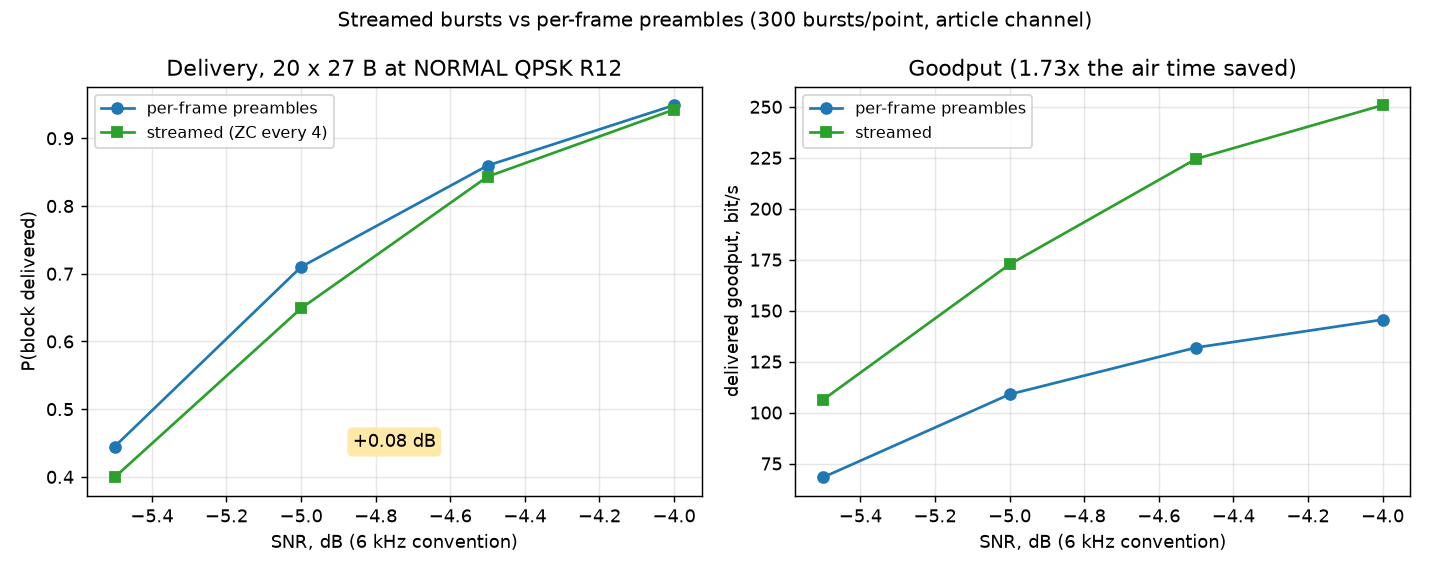
\includegraphics[width=\textwidth]{images/stream_mode.png}
    \caption{Streamed bursts against per-frame preambles
             (\texttt{experiments/stream\_mode.py}).  Delivery is
             scored per block, so the comparison is packets delivered
             rather than frames sent.}
    \label{fig:stream_mode}
\end{figure}

Three properties took measurement rather than reasoning to establish.
First, \textbf{the Zadoff--Chu resync is not what holds the stream
together}: with resync disabled entirely a 24\,s stream decodes at the
same packet-error rate, because the per-symbol frequency search and the
pilot channel estimate already do all the tracking.  The resync earns
its place on sample-clock offset --- a 32-sample cyclic prefix slips in
$\approx$133\,s at 20\,ppm --- and as a re-entry point for a receiver
that missed the opening preamble.  Second, \textbf{failures do not
cascade}: block offsets are deterministic, so a block that fails its
CRC costs exactly that block, and its raw LLRs are retained for chase
combining on the retransmission.  Third, \textbf{the cost grows with
burst length}: a 5-block EXTREME burst measured $\approx$0.35\,dB for
only $1.21\times$, which is why streaming is recommended at NORMAL
rungs and not at the modes where decibels are most expensive.

One invariant is easy to violate: the clip-and-filter threshold is a
\emph{whole-waveform} RMS, so a burst is not the concatenation of
separately built frames.  A one-block burst with no resync is
bit-identical to an ordinary frame, and both the float and fixed-point
test suites assert exactly that.

\subsection{Transmit Chain}

Figure~\ref{fig:tx_chain} shows the transmit chain
(\texttt{Transceiver.build\_frame}).  Packet bits (with CRC) are
FEC-encoded, zero-padded to a whole number of OFDM symbols
\emph{before} interleaving, interleaved over the 16 data carriers,
scrambled by a 15-bit LFSR, mapped (BPSK/QPSK/16-QAM Gray), and
assembled into OFDM symbols with the ZC pilots and a Hermitian mirror
so the time-domain signal is real.  After tiling and CP insertion the
preamble is prepended and a clip-and-filter stage (clip at
RMS+6\,dB, low-pass at 3\,kHz) bounds the PAPR.

\begin{figure}[H]
    \centering
    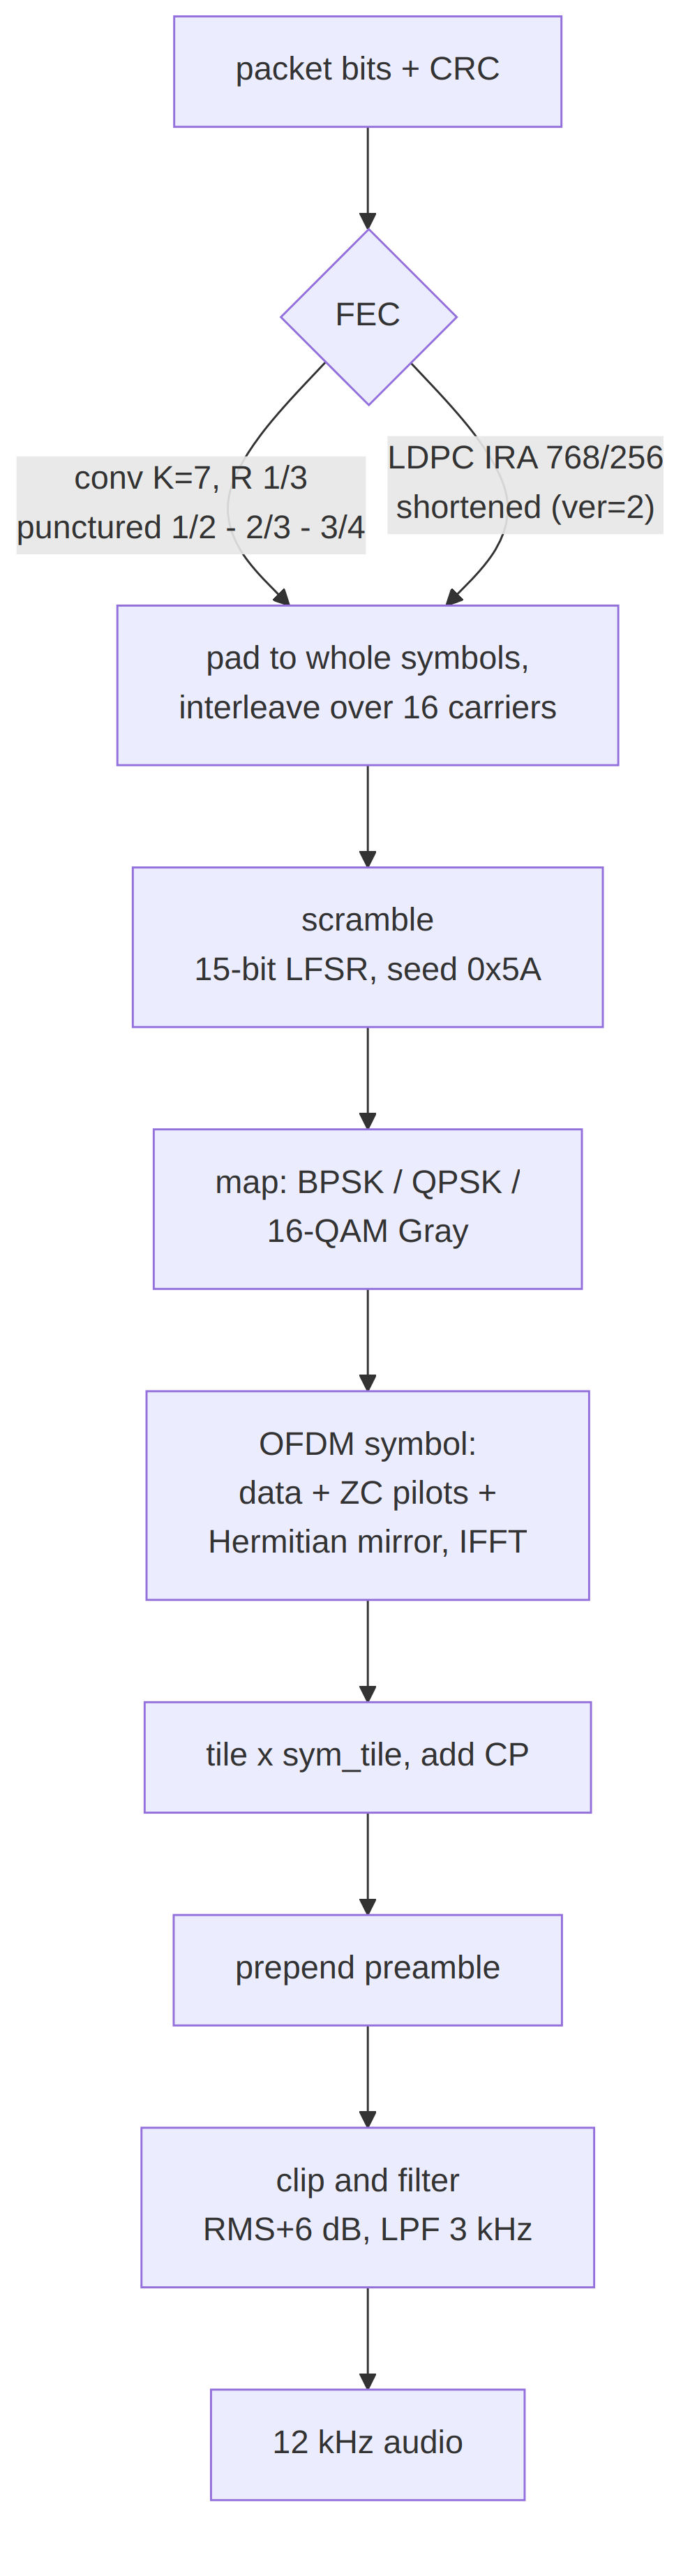
\includegraphics[width=0.62\textwidth,height=0.55\textheight,keepaspectratio]{images/tx_chain.png}
    \caption{Transmit chain.}
    \label{fig:tx_chain}
\end{figure}

Two ordering invariants are easy to break and worth stating: TX applies
interleave \emph{then} scramble, so RX must descramble \emph{then}
deinterleave; and because the FEC block is padded to whole symbols
before interleaving, RX must crop the deinterleaved stream back to the
codec's block length before decoding.

\subsection{Receive Chain}

Figure~\ref{fig:rx_chain} shows the receive chain
(\texttt{Transceiver.demod\_frame}).  After the analytic-signal
transform, synchronization runs in three stages (detailed in
Section~\ref{sec:sync}); the demodulator then processes each tiled
symbol: CP removal and coherent tile accumulation (with per-symbol
phase tracking), FFT, pilot-based channel estimation (zero-forcing
estimate at the pilots, Wiener smoothing with an exponential
frequency-correlation model of length 8 bins, MMSE equalization), and
LLR formation weighted by the per-carrier symbol SNR, clipped to
$\pm 20$.  One convention is load-bearing across four modules: LLR
sign is \textbf{positive = logical 1}, consistent with the article's
BPSK mapping table (the article's prose states the opposite of its own
code).

\begin{figure}[H]
    \centering
    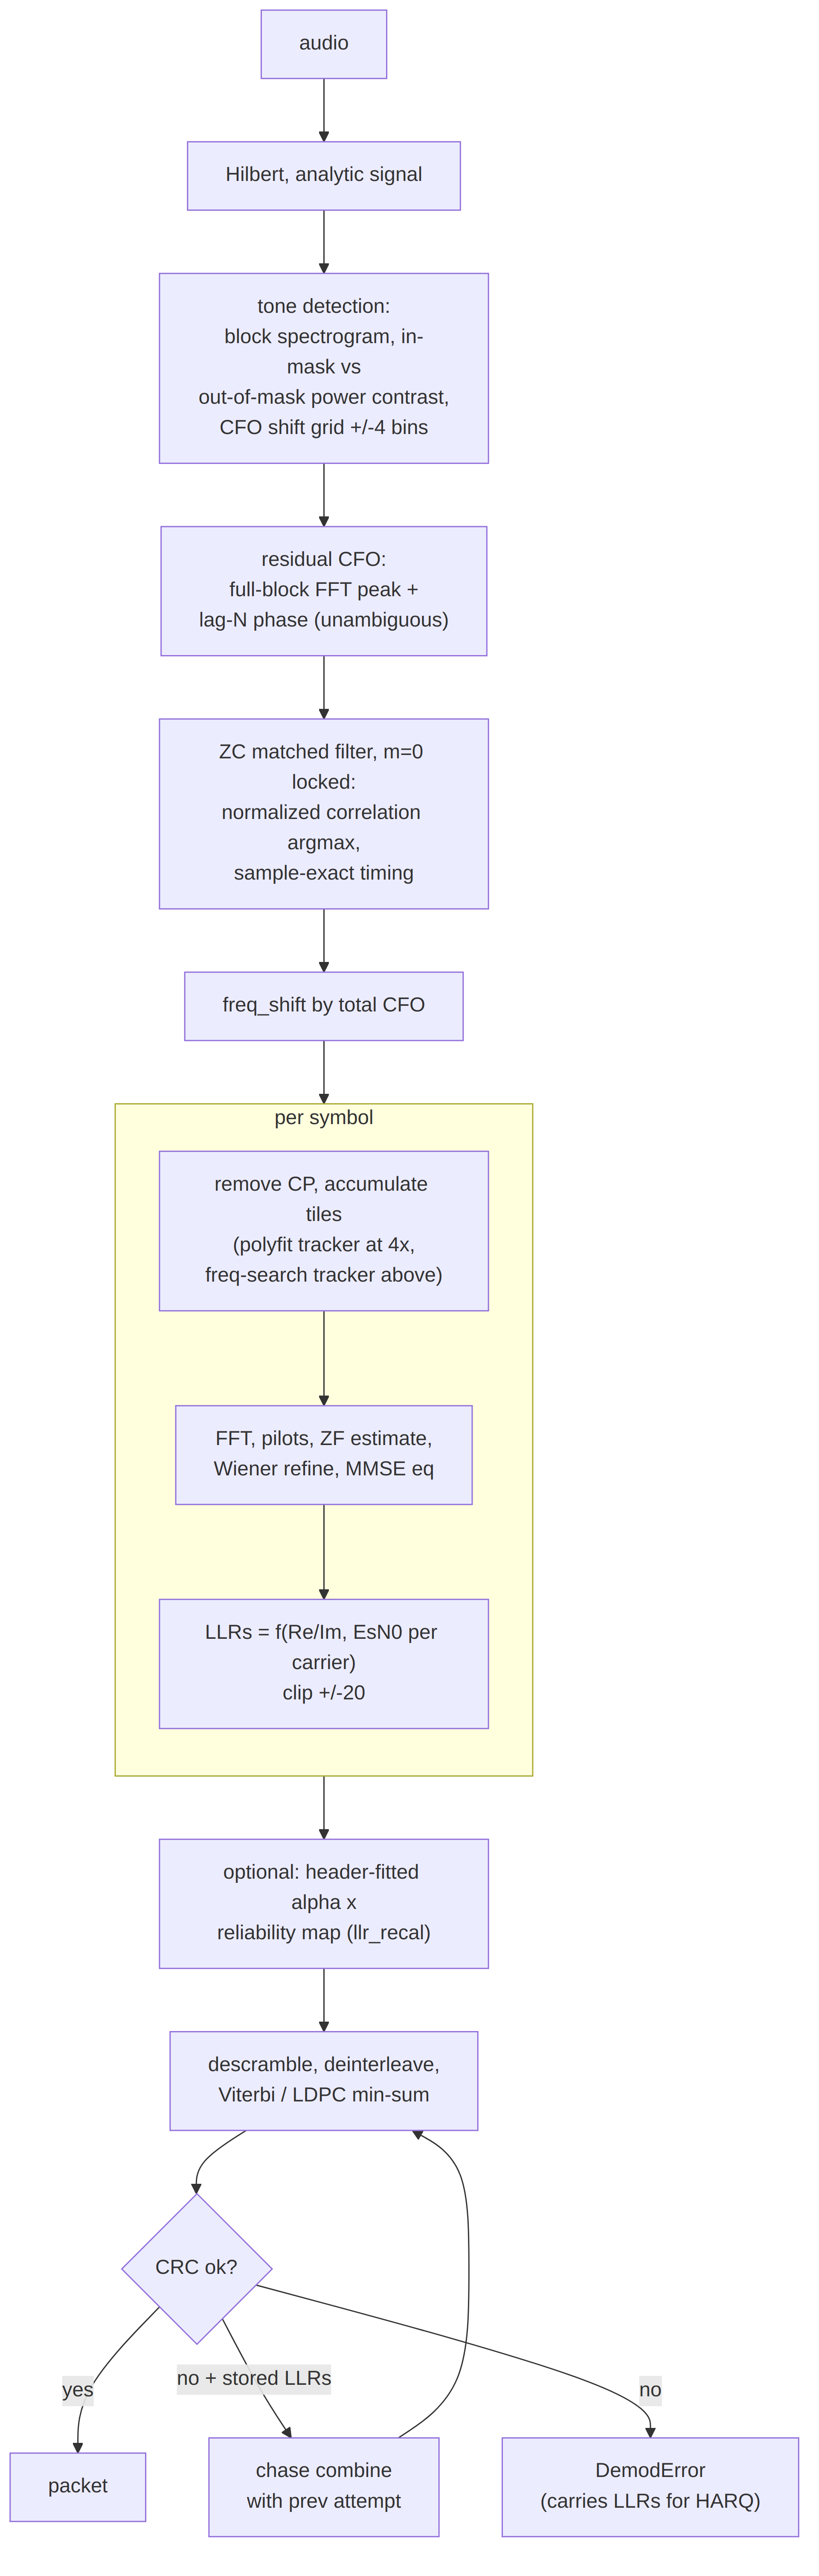
\includegraphics[width=0.72\textwidth,height=0.6\textheight,keepaspectratio]{images/rx_chain.png}
    \caption{Receive chain, including the opt-in recalibration stage
             (Section~\ref{sec:llr}) and the HARQ path
             (Section~\ref{sec:coding}).}
    \label{fig:rx_chain}
\end{figure}

A CRC failure does not simply discard the frame: the
\texttt{DemodError} exception carries the decoded header and the
data-block LLRs, which is what makes the chase-combining HARQ of
Section~\ref{sec:coding} possible without any extra signalling.

\subsection{Soft Demodulation: from Symbols to LLRs}
\label{sec:llr_math}

This subsection states exactly what the demodulator computes
(\texttt{OFDMModem.demodulate\_symbol\_cp\_soft}).  After tile
accumulation and FFT, each data carrier $k$ of a symbol obeys
\begin{equation}
    Y_k = H_k S_k + N_k,
    \qquad N_k \sim \mathcal{CN}(0, \sigma^2),
\end{equation}
where $H_k$ is the channel coefficient and $S_k$ the transmitted
constellation point.  With $\hat{H}_k$ the Wiener-smoothed pilot
estimate, the MMSE equalizer output is
\begin{equation}
    \hat{S}_k \;=\;
    \frac{Y_k\,\hat{H}_k^{*}}{|\hat{H}_k|^{2} + \hat{\sigma}^{2}} .
    \label{eq:mmse}
\end{equation}
The noise power $\hat\sigma^2$ is tracked decision-directed: the
mean-square error of $\hat S_k$ against the nearest constellation
point (per axis for BPSK/QPSK; against the sliced 16-QAM grid for
$\mu=4$), referred back through the channel by the mean
$|\hat H_k|^2$, and smoothed with an exponential filter
($\alpha = 0.1$) across symbols.  The per-carrier symbol SNR
\begin{equation}
    \rho_k \;=\; \frac{|\hat{H}_k|^{2}}{\hat{\sigma}^{2}}
\end{equation}
weights every LLR, so bits on faded carriers enter the decoder as
weak evidence rather than as confident errors.

The log-likelihood ratio of a bit $b$ is defined here as
\begin{equation}
    L(b) \;=\;
    \ln \frac{P(b = 1 \mid \hat{S})}{P(b = 0 \mid \hat{S})},
\end{equation}
i.e.\ \textbf{positive LLR means logical~1} --- the load-bearing sign
convention noted above.  Under the max-log approximation
$\ln \sum_i e^{x_i} \approx \max_i x_i$, the general form
\begin{equation}
    L(b_i) \;\approx\; \rho_k
    \Bigl( \min_{s \in \mathcal{S}_0^{(i)}} |\hat{S}_k - s|^2
         - \min_{s \in \mathcal{S}_1^{(i)}} |\hat{S}_k - s|^2 \Bigr)
\end{equation}
collapses to closed forms per modulation (as implemented; overall
scale is immaterial to the scale-invariant Viterbi and min-sum
decoders, but the \emph{shape} across carriers and bit positions is
what Section~\ref{sec:llr} calibrates):
\begin{align}
    \text{BPSK:}\quad
        & L = 4\,\rho_k \operatorname{Re}\hat{S}_k, \\
    \text{QPSK:}\quad
        & L_I = 2\,\rho_k \operatorname{Re}\hat{S}_k,
    \qquad L_Q = 2\,\rho_k \operatorname{Im}\hat{S}_k, \\
    \text{16-QAM (Gray, unit } a = g/\sqrt{10}\text{):}\quad
        & L_{b_0} = 2\,\rho_k \operatorname{Re}\hat{S}_k / g,
    \qquad L_{b_1} = 2\,\rho_k
        \bigl(2a - |\operatorname{Re}\hat{S}_k|\bigr) / g,
    \label{eq:qam_llr}
\end{align}
with the imaginary-axis pair $L_{b_2}, L_{b_3}$ analogous, and $g$ the
per-symbol gain estimate.  The 16-QAM forms are the piecewise-linear
max-log metrics of the Gray mapping: the outer bit ($b_0$) is the axis
sign, the inner bit ($b_1$) discriminates inner from outer amplitude
levels, changing sign at $|\!\operatorname{Re}\hat S| = 2a$.  All LLRs
are clipped to $\pm 20$ before decoding.

\subsection{Symbol Demodulation, Exactly: Tile Accumulation Across the Modes}
\label{sec:demod_exact}

The previous subsection gives the mathematics of one OFDM symbol.  This
one gives the procedure as the code executes it, from the detected
frame to a block of LLRs, in the same self-contained form as
\S\ref{sec:zc}: Table~\ref{tab:demod_notation} defines the symbols,
Algorithm~\ref{alg:frame_demod} is the frame loop, Algorithms
\ref{alg:acc_poly} and~\ref{alg:acc_search} are the two ways the float
receiver collapses a tiled symbol into one spectrum (the polynomial
phase tracker at NORMAL, the gated frequency search at ROBUST and
EXTREME), Algorithm~\ref{alg:soft_demod} turns a spectrum into LLRs,
Algorithm~\ref{alg:demod_int} is the integer form the fixed-point twin
and the C port share for every mode, and Algorithm~\ref{alg:demod_prims}
holds the two integer primitives it needs beyond those of
Algorithm~\ref{alg:zc_prims}.

\begin{table}[H]
    \centering
    \caption{Notation of Algorithms~\ref{alg:frame_demod}--\ref{alg:demod_prims}
             (symbols of Table~\ref{tab:zc_notation} carry over).}
    \label{tab:demod_notation}
    \small
    \begin{tabular}{@{}lp{3.4cm}p{8.4cm}@{}}
    \toprule
    \textbf{Symbol} & \textbf{Value} & \textbf{Meaning} \\
    \midrule
    $T$ & 4 / 16 / 64 & tiles per symbol (\texttt{sym\_tile}) \\
    $S$ & $\mathrm{CP} + TN$ & symbol length in samples: 544 / 2080 / 8224 \\
    $D$ & $S/f_s$ & symbol duration: 45.3 / 173 / 685\,ms \\
    $\mathcal{K}$ & bins 3..25 & the 23 loaded (channel) bins \\
    $\mathcal{P}$, $\mathcal{D}$ & 7, 16 of $\mathcal{K}$ & pilot carriers; data carriers (local indices into $\mathcal{K}$) \\
    $p_k$ & Eq.~\eqref{eq:zc}, $u{=}3$, $N{=}7$ & pilot reference values, $|p_k| = 1$ \\
    $\mu$ & 1 / 2 / 4 & bits per carrier: BPSK / QPSK / 16-QAM \\
    $R$ & 8 / 8 / 25\,Hz & residual-CFO search range (\texttt{freq\_range}) \\
    $\Delta_f$ & $0.25/D$ (float); $0.125/D$ (int) & search step: a quarter (eighth) cycle over one symbol \\
    $\mathcal{G}$ & $\{-R, -R{+}\Delta_f, \ldots, R\}$ & the grid: 4 / 12 / 138 points (float), 7 / 23 / 275 (int) \\
    $T_c$ & $\max(4, T/4)$ & tiles used by the coarse pass: 4 / 4 / 16 \\
    $\gamma$ & 2.25 (36 in Q4) & coarse gate: top-1 over median energy contrast \\
    $\ell_c$ & 8 bins & Wiener frequency-correlation length \\
    $\alpha$ & 0.1 & noise-variance smoothing (float) \\
    $\sigma^2$ & scalar & tracked noise variance, in units of $|H|^2$ \\
    $\rho_k$ & scalar & per-carrier $E_s/N_0$, $|H_k|^2/\sigma^2$ \\
    $c$ & $\pm 20$ & LLR clip (float) \\
    $B$ & 13 & BFP target bits in the demodulator's FFT \\
    $e$ & integer & block exponent of a spectrum: values scale as $2^{e}$, energies as $2^{2e}$ \\
    $q$ & 6 / 8 bits & LLR quantization: $\mu \le 2$ / $\mu = 4$ \\
    \bottomrule
    \end{tabular}
\end{table}

\begin{algorithm}[H]
\caption{Float frame demodulation (\texttt{Transceiver.demod\_frame}), from detection to data LLRs.}
\label{alg:frame_demod}
\begin{algorithmic}[1]
\Require real audio $s[n]$; a modem $m$ of the frame's mode
\Ensure data-block LLRs, per-carrier and mean $E_s/N_0$, header
\State $x \gets \mathrm{hilbert}(s)$ \Comment{analytic signal}
\State $(\mathrm{start}, \mathrm{cfo}) \gets m.\textsc{DetectPreamble}(x)$; \textbf{if} \textsc{None}: \textbf{raise} \textsc{DemodError} \Comment{\S\ref{sec:zc}}
\State $y[n] \gets x[n]\, e^{-2\pi j\, \mathrm{cfo}\, n/f_s}$; append $S$ zeros \Comment{derotate the frame; slack for a slip on the last symbol}
\State $m.\mathrm{mapper} \gets \mathrm{BPSK}$;\quad $n_h \gets \lceil 93 / 16 \rceil = 6$ \Comment{header: 93 coded bits, 16 per symbol}
\For{$i = 0..n_h{-}1$} \Comment{header symbols}
    \State $(\rho, \bar\rho, \Lambda_i) \gets \textsc{SoftDemod}(m, \textsc{Accumulate}(m, y[\mathrm{start} + iS .. \mathrm{start} + (i{+}1)S)))$
\EndFor
\State $\mathrm{hdr} \gets \textsc{Viterbi}_{1/3}([\Lambda_0 .. \Lambda_{n_h-1}])$; decode fields, check CRC-8 \Comment{Section~\ref{sec:coding}}
\State $\alpha_{\mathrm{llr}} \gets \mathrm{clip}\big(2\,\mathbb{E}[\Lambda x]/\mathrm{Var}[\Lambda x],\ 0.05,\ 4\big)$ over the 96 header positions \Comment{temperature, \S\ref{sec:llr}}
\State $\mathrm{pos} \gets \mathrm{start} + n_h S$;\quad $m.\mathrm{mapper} \gets \mathrm{hdr.mod}$
\State codec $\gets$ LDPC if $\mathrm{hdr.ver} = 2$ else conv at rate $\mathrm{hdr.spd}$
\State $n_d \gets \lceil \mathrm{codec.coded\_bits}(\mathrm{hdr.len}) / (16\mu) \rceil$
\For{$i = 0..n_d{-}1$} \Comment{data symbols, same two steps}
    \State $(\rho^{(i)}, \bar\rho^{(i)}, \Lambda_i) \gets \textsc{SoftDemod}(m, \textsc{Accumulate}(m, y[\mathrm{pos} + iS .. \mathrm{pos} + (i{+}1)S)))$
\EndFor
\State $\Lambda \gets \alpha_{\mathrm{llr}} \cdot [\Lambda_0 .. \Lambda_{n_d-1}]$; \textbf{if} recalibration on \textbf{and} $\mu \le 2$: $\Lambda \gets \textsc{ReliabilityMap}(\Lambda)$ \Comment{\S\ref{sec:llr}}
\State \Return $\Lambda$, $\mathrm{mean}_i\, \rho^{(i)}$, $\mathrm{mean}_i\, \bar\rho^{(i)}$, hdr
\end{algorithmic}
\end{algorithm}

\textsc{Accumulate} is where the modes differ.  Every tiled symbol is
$T$ back-to-back repeats of one $N$-sample OFDM symbol behind one CP;
the receiver must add the repeats coherently, and the residual carrier
offset that the preamble left (a few hertz) rotates each repeat by a
little more than the last.  At NORMAL the four repeats are long enough
in SNR to measure their pairwise phases, and a polynomial fitted to
those phases removes the rotation (Algorithm~\ref{alg:acc_poly}).  At
ROBUST and EXTREME the pairwise phases are noise at the operating
point, so the receiver instead \emph{hypothesises} the residual
frequency, derotates the whole symbol by each candidate, and keeps the
one that concentrates the most energy in the loaded bins
(Algorithm~\ref{alg:acc_search}) --- spending the whole symbol's
energy on the decision instead of a tile's.  The grid step is a quarter
cycle over the symbol, so the winning hypothesis leaves at most
$\sim\pi/4$ of phase ramp across the accumulation.

\begin{algorithm}[H]
\caption{\textsc{Accumulate}, NORMAL ($T = 4$): polynomial phase tracker (\texttt{TiledOFDMModem.\_demodulate\_signal}).}
\label{alg:acc_poly}
\begin{algorithmic}[1]
\Require the $TN$ samples after the CP, as tiles $r_0 .. r_{T-1}$ of $N$
\Ensure one $N$-point spectrum
\State $s_{\max} \gets \min(3, T{-}1)$
\For{$d = 1..s_{\max}$, $i = 0..T{-}1{-}d$} $\ \theta_{i,i+d} \gets \angle \sum_n r_i[n]\, \overline{r_{i+d}[n]}$ \Comment{pairwise tile phases} \EndFor
\State $X \gets [0]$;\ $Y \gets [0]$ \Comment{(tile index, phase) samples for the fit}
\For{$t = 1..T{-}1$}
    \State \textbf{if} $t \le s_{\max}$: append $(t, -\theta_{0,t})$ \Comment{direct estimate}
    \State append $\big(t,\ -\sum_{i<t} \theta_{i,i+1}\big)$ \Comment{chained step-1 estimate}
    \State \textbf{if} $t \ge 2$: append $\big(t,\ -(\theta_{t-2,t} + \theta_{t-4,t-2} + \cdots)\big)$, ending with $\theta_{0,1}$ if $t$ is odd \Comment{chained step-2}
\EndFor
\State $(a_2, a_1, a_0) \gets \mathrm{polyfit}(X, Y, 2)$;\quad $\varphi_t \gets a_2 t^2 + a_1 t$ \Comment{degree-2 fit, anchored at tile 0}
\State $\bar r[n] \gets \frac{1}{T} \sum_{t=0}^{T-1} r_t[n]\, e^{-j\varphi_t}$ \Comment{derotate each tile onto the first, average}
\State \Return $\mathrm{FFT}_N(\bar r)$
\end{algorithmic}
\end{algorithm}

\begin{algorithm}[H]
\caption{\textsc{Accumulate}, ROBUST and EXTREME: gated two-stage frequency search (\texttt{\_demodulate\_freq\_search}).}
\label{alg:acc_search}
\begin{algorithmic}[1]
\Require the $TN$ samples after the CP as $z[n]$; grid $\mathcal{G}$
\Ensure one $N$-point spectrum
\Function{Energy}{$f$, $n_t$} \Comment{derotate the first $n_t$ tiles by $f$, accumulate, measure the loaded bins}
    \State $d[n] \gets z[n]\, e^{-2\pi j f n / f_s}$, $n < n_t N$;\quad $\bar d[n] \gets \frac{1}{n_t}\sum_{t < n_t} d[tN + n]$
    \State $Z \gets \mathrm{FFT}_N(\bar d)$;\quad \Return $\sum_{k \in \mathcal{K}} |Z[k]|^2$, $Z$
\EndFunction
\State $\mathcal{I} \gets$ all indices of $\mathcal{G}$
\If{$|\mathcal{G}| > 9$} \Comment{coarse pass only where a grid is worth pruning}
    \State $E_c[k] \gets \textsc{Energy}(\mathcal{G}[k], T_c).\mathrm{energy}$ for $k = 0, 4, 8, \ldots$ \Comment{every 4th point on $T_c$ tiles}
    \State rank $E_c$ descending; $\mathrm{med} \gets$ its median (or 1)
    \If{$E_c^{\mathrm{top}} / \mathrm{med} \ge \gamma$} $\ \mathcal{I} \gets \bigcup_{\text{top-3 } k} \{k{-}5 .. k{+}5\} \cap [0, |\mathcal{G}|)$ \Comment{decisive: shortlist} \EndIf
    \Statex \hspace{\algorithmicindent} otherwise keep the full grid \Comment{the gate keeps the shortcut lossless at the edge}
\EndIf
\State $\mathrm{best} \gets (E{=}-1, Z{=}\varnothing)$
\For{$k \in \mathcal{I}$} $\ (E, Z) \gets \textsc{Energy}(\mathcal{G}[k], T)$;\ \textbf{if} $E > \mathrm{best}.E$: $\mathrm{best} \gets (E, Z)$ \EndFor
\State \Return $\mathrm{best}.Z$
\end{algorithmic}
\end{algorithm}

\begin{algorithm}[H]
\caption{\textsc{SoftDemod}: spectrum to LLRs (\texttt{OFDMModem.demodulate\_symbol\_cp\_soft}), float.}
\label{alg:soft_demod}
\begin{algorithmic}[1]
\Require spectrum $Z[k]$; mapper $\mu$; pilot values $p$; carrier sets $\mathcal{K}, \mathcal{P}, \mathcal{D}$
\Ensure $\rho_k$ (per data carrier), $\bar\rho$, LLR vector $\Lambda$ of length $16\mu$
\State $\hat H^{\mathrm{p}}_j \gets Z[\mathcal{P}_j] / p_j$, $j = 0..6$ \Comment{ZF at the pilots}
\State $\hat H^{0}_k \gets$ linear interpolation of $\mathrm{Re}, \mathrm{Im}\, \hat H^{\mathrm{p}}$ over $k \in \mathcal{K}$ \Comment{initial estimate}
\State $\hat x^{0}_k \gets Z[k] / (\hat H^{0}_k + 10^{-6})$ for $k \in \mathcal{D}$ \Comment{ZF equalize}
\State $\hat s^{0}_k \gets$ nearest constellation point to $\hat x^{0}_k$ ($\mathrm{sign}$; $\mathrm{sign}/\sqrt2$; 16-QAM levels $\{\pm1,\pm3\}/\sqrt{10}$)
\State $\sigma^2 \gets \mathrm{clip}\big(\mathrm{mean}_k |\hat x^0_k - \hat s^0_k|^2 \cdot \mathrm{mean}_k |\hat H^0_k|^2,\ 10^{-6},\ 60\big)$ \Comment{initial noise variance}
\State $r_{hp}[k,j] \gets e^{-|k - \mathcal{P}_j|/\ell_c}$;\quad $r_{pp}[i,j] \gets e^{-|\mathcal{P}_i - \mathcal{P}_j|/\ell_c}$ \Comment{exponential correlation model}
\State $\hat H_k \gets \Big(r_{hp}\,\big(r_{pp} + \tfrac{\sigma^2}{\mathrm{mean}_j|\hat H^{\mathrm{p}}_j|^2} I\big)^{-1} \hat H^{\mathrm{p}}\Big)_k$ \Comment{Wiener estimate over $\mathcal{K}$}
\State $\hat x_k \gets Z[k]\, \overline{\hat H_k} \big/ (|\hat H_k|^2 + \sigma^2)$ for $k \in \mathcal{D}$ \Comment{MMSE equalize}
\State decision-directed residual: $\hat s_k \gets$ nearest point (with per-axis amplitude for $\mu \le 2$, gain $g = \sqrt{\mathrm{mean}|\hat x_k|^2}$, $a = g/\sqrt{10}$ for $\mu = 4$);\quad $v \gets \mathrm{mean}_k |\hat x_k - \hat s_k|^2$
\State $\sigma^2 \gets \max\big(\alpha\, v \cdot \mathrm{mean}_k|\hat H_k|^2 + (1 - \alpha)\, \sigma^2,\ 10^{-6}\big)$ \Comment{one-pole update}
\State $\rho_k \gets |\hat H_k|^2 / \sigma^2$;\quad $\bar\rho \gets \mathrm{mean}_k|\hat H_k|^2 / \sigma^2$
\State $\mu = 1$: $\Lambda \gets 4\rho_k \mathrm{Re}\,\hat x_k$;\quad $\mu = 2$: $\Lambda \gets [2\rho_k \mathrm{Re}\,\hat x_k,\ 2\rho_k \mathrm{Im}\,\hat x_k]$ interleaved
\State $\mu = 4$: $\Lambda \gets \big[\,2\rho_k \mathrm{Re}\,\hat x_k/g,\ \ 2\rho_k(2a - |\mathrm{Re}\,\hat x_k|)/g,\ \ 2\rho_k \mathrm{Im}\,\hat x_k/g,\ \ 2\rho_k(2a - |\mathrm{Im}\,\hat x_k|)/g\,\big]$ \Comment{Eq.~\eqref{eq:qam_llr}}
\State \Return $\rho_k$, $\bar\rho$, $\mathrm{clip}(\Lambda, -c, c)$
\end{algorithmic}
\end{algorithm}

The integer receiver (Algorithm~\ref{alg:demod_int}) differs from the
float chain in three ways that Section~\ref{sec:fixed} motivates and
Table~\ref{tab:fixed_vs_float} lists; they are visible in the listing.
It uses the frequency search for \emph{every} mode, NORMAL included,
with a \emph{slew-limited tracker}: the full grid (through the gated
coarse pass) on the first symbol of a frame, then $\pm 2$ grid steps
around the previous symbol's winner, because the residual drift is
smooth and a per-symbol argmax is noisy.  It \emph{sums} the tiles
instead of averaging them and carries the growth in a block exponent,
so the FFT input always fills 13 bits.  And it produces
\emph{matched-filter} LLRs, $Y_k \overline{\hat H_k}$, with no division
and no noise estimate: since $Y_k \overline{\hat H_k} = |\hat H_k|^2
x_k + \text{noise}$, this is the float LLR $4\rho_k \mathrm{Re}\,\hat
x_k = 4\,\mathrm{Re}(Y_k \overline{\hat H_k})/\sigma^2$ up to the
per-symbol constant $\sigma^2$, which the scale-invariant Viterbi and
min-sum decoders do not need --- the per-carrier SNR weighting is
already inside the product.  What the integer chain gives up is the
per-symbol \emph{absolute} LLR scale, which is why its calibrated mode
(Section~\ref{sec:fixed}) exists for HARQ combining and why the SNR
estimator of \S\ref{sec:cport_snrcal} is a separate statistic.

\begin{algorithm}[H]
\caption{Integer symbol demodulation, all modes (fixed-point twin and C port).}
\label{alg:demod_int}
\begin{algorithmic}[1]
\Require int16 $I, Q$; symbol start $\mathrm{pos}$; frame CFO word $w_0$; $\mu$; grid words $\mathcal{W}_{\mathcal G}$; tracker state $h_{\mathrm{last}}$ (none at frame start)
\Ensure block LLRs $\Lambda$ (int), block exponent $e_b$
\Function{Spectrum}{$k$, $n_t$} \Comment{derotate by $w_0 + \mathcal{W}_{\mathcal G}[k]$, sum $n_t$ tiles, BFP FFT}
    \State $w \gets \mathcal{W}_{\mathcal G}[k]$;\quad $\phi_0 \gets (w_0 + w)\,\mathrm{pos} \bmod 2^{32}$ \Comment{phase continuous across symbols}
    \State $(d_I, d_Q) \gets \textsc{NcoDerotate}(I[\mathrm{pos} .. \mathrm{pos}{+}\mathrm{CP}{+}n_t N),\ Q[\ldots],\ w_0 + w,\ \phi_0)$
    \State $A_I[n] \gets \sum_{t < n_t} d_I[\mathrm{CP} + tN + n]$;\quad $A_Q[n] \gets \sum_{t < n_t} d_Q[\mathrm{CP} + tN + n]$ \Comment{tiles summed}
    \State $(Z_r, Z_i, e) \gets \textsc{FftBfp}(A_I, A_Q, B)$;\quad $E \gets \sum_{k \in \mathcal{K}} Z_r[k]^2 + Z_i[k]^2$
    \State \Return $(E, Z_r, Z_i, e)$
\EndFunction
\Statex
\State \textbf{hypothesis window:}
\If{$h_{\mathrm{last}}$ is none} \Comment{first symbol of the frame}
    \State $\mathcal{I} \gets$ all of $\mathcal{G}$
    \If{$|\mathcal{G}| > 9$} \Comment{coarse pass of Algorithm~\ref{alg:acc_search}, integer form}
        \State $E_c[k] \gets \textsc{Spectrum}(k, T_c)$ for $k = 0, 4, 8, \ldots$; align: $E \gg \min(2(e - e_{\min}), 62)$
        \State \textbf{if} $(E_c^{\mathrm{top}} \ll 4) / \mathrm{med} \ge 36$: $\mathcal{I} \gets$ the top-3 $\pm5$ windows \Comment{$\gamma$ as 36 in Q4}
    \EndIf
\Else\ $\mathcal{I} \gets [h_{\mathrm{last}} - 2,\ h_{\mathrm{last}} + 2] \cap [0, |\mathcal{G}|)$ \Comment{slew-limited tracker}
\EndIf
\State $\mathrm{cand}_k \gets \textsc{Spectrum}(k, T)$ for $k \in \mathcal{I}$;\quad $e_{\min} \gets \min_k e_k$
\State $k^\star \gets \arg\max_k \big(E_k \gg \min(2(e_k - e_{\min}), 62)\big)$ \Comment{energies on a common exponent}
\State $(Z_r, Z_i, e) \gets \mathrm{cand}_{k^\star}$;\quad $h_{\mathrm{last}} \gets k^\star$
\Statex
\State \textbf{channel estimate:} $\hat H^{\mathrm{p}}_j \gets \textsc{RshiftRound}\big(Z[\mathcal{P}_j] \cdot \overline{p_j}^{\,\mathrm{Q15}},\ 15\big)$, $j = 0..6$ \Comment{conjugate ROM}
\State $\hat H_k \gets \big(\hat H^{\mathrm{p}}_{lo}\,(2^{15} - \omega_k) + \hat H^{\mathrm{p}}_{hi}\,\omega_k\big) \gg 15$, $k \in \mathcal{K}$ \Comment{Q15 weight ROM}
\Statex
\State \textbf{LLRs} (matched filter, scale $\propto 2^{2e}$), $k \in \mathcal{D}$: $\Lambda^I_k \gets Z_r \hat H_r + Z_i \hat H_i$;\quad $\Lambda^Q_k \gets Z_i \hat H_r - Z_r \hat H_i$
\State $\mu = 1$: $\Lambda \gets \Lambda^I$;\quad $\mu = 2$: $\Lambda \gets [\Lambda^I_k, \Lambda^Q_k]$ interleaved
\State $\mu = 4$: $h2_k \gets \hat H_r^2 + \hat H_i^2$;\quad $\varrho \gets \big((\sum_k |\Lambda^I_k| + |\Lambda^Q_k|) \ll 8\big) \big/ (2 \sum_k h2_k)$
\Statex \hspace{\algorithmicindent} $\tau_k \gets (h2_k\, \varrho) \gg 8$;\quad $\Lambda \gets [\Lambda^I_k,\ \tau_k - |\Lambda^I_k|,\ \Lambda^Q_k,\ \tau_k - |\Lambda^Q_k|]$ \Comment{$\mathbb{E}|x_I| = 2a$}
\State \Return $\Lambda$, $e$
\Statex
\State \textbf{block:} for symbols $i = 0..n{-}1$ collect $(\Lambda_i, e_i)$ as above;\quad $e_{\min} \gets \min_i e_i$
\State $\Lambda \gets [\Lambda_i \gg 2(e_i - e_{\min})]_i$;\quad \Return $\Lambda$, $e_b = 2 e_{\min}$ \Comment{block on a common exponent}
\State \textbf{then} $\textsc{Quantize}(\Lambda, q)$ with $q = 8$ if $\mu = 4$ else $6$ \Comment{before the decoder}
\end{algorithmic}
\end{algorithm}

\begin{algorithm}[H]
\caption{Integer primitives of Algorithm~\ref{alg:demod_int} (\texttt{fixed/fft.py}, \texttt{fixed/fxp.py}; bit-identical in \texttt{cport/src/fft.c}).}
\label{alg:demod_prims}
\begin{algorithmic}[1]
\Function{FftBfp}{$x_r[0..N)$, $x_i[0..N)$, $B$} \Comment{block floating point around a scaled FFT}
    \State $m \gets \max(\max_n |x_r[n]|,\ \max_n |x_i[n]|,\ 1)$;\quad $e \gets B - \mathrm{bitlength}(m)$ \Comment{priority encoder on the block max}
    \State \textbf{if} $e \ge 0$: $x \gets x \ll e$ \textbf{else} $x \gets \textsc{RshiftRound}(x, -e)$ \Comment{fill $B$ bits}
    \State \Return $\textsc{FftFixed}(x_r, x_i)$, $e$ \Comment{spectrum is $2^{e}\times$ the unscaled transform}
\EndFunction
\Statex
\Function{FftFixed}{$x_r$, $x_i$} \Comment{radix-2 DIT, Q15 twiddles, per-stage $\gg 1$ = built-in $1/N$}
    \State ROM: $W_r[k] \gets \mathrm{round}(32767 \cos(2\pi k/N))$,\ $W_i[k] \gets \mathrm{round}(-32767 \sin(2\pi k/N))$, $k < N/2$
    \State bit-reverse the input order;\quad $h \gets 1$
    \While{$h < N$}
        \For{each butterfly pair $(i_0, i_1 = i_0 + h)$ with twiddle index $k \cdot N/2h$}
            \State $t_r \gets \textsc{RshiftRound}(x_r[i_1] W_r - x_i[i_1] W_i,\ 15)$;\quad $t_i \gets \textsc{RshiftRound}(x_r[i_1] W_i + x_i[i_1] W_r,\ 15)$
            \State $x[i_1] \gets \textsc{RshiftRound}(x[i_0] - t,\ 1)$;\quad $x[i_0] \gets \textsc{RshiftRound}(x[i_0] + t,\ 1)$ \Comment{both components}
        \EndFor
        \State $h \gets 2h$
    \EndWhile
    \State \Return $x_r, x_i$
\EndFunction
\Statex
\Function{Quantize}{$\Lambda$, $q$} \Comment{peak-normalized to $q$ bits}
    \State $\mathrm{peak} \gets \max_i |\Lambda_i|$;\quad $s \gets \max(0,\ \mathrm{bitlength}(\mathrm{peak}) - (q - 1))$
    \State \Return $\mathrm{clip}(\Lambda \gg s,\ -(2^{q-1} - 1),\ 2^{q-1} - 1)$ \Comment{$\pm31$ at 6 bits, $\pm127$ at 8}
\EndFunction
\end{algorithmic}
\end{algorithm}

Three consequences of Algorithm~\ref{alg:demod_int} are measured
elsewhere in this report and are worth connecting to their lines.  The
peak-normalized 6-bit quantization (\textsc{Quantize}) is what makes
the fixed receiver \emph{beat} the recalibrated float receiver at
$-9/-10$\,dB: it compresses the LLR range the way the monotone map
does, for free (Section~\ref{sec:fixed}).  The block exponent
$e_b$ and the $2^{2e}$ energy scaling are the invariant every energy
comparison in the chain must respect --- the hypothesis argmax
aligns exponents before comparing, and forgetting to do so is
one of the three integer-domain bugs of Section~\ref{sec:fixed}'s debug
lore.  And the tracker's $\pm 2$ window is the reason the EXTREME
demodulator costs 856\,Mcycles per frame rather than the 275-hypothesis
grid's worth on every symbol (Table~\ref{tab:cport_stages}): the grid is
paid once per frame, on the first symbol, and only there through the
gated coarse pass.

\subsection{Tone Detection, Exactly: the Newman Preamble Across the Modes and Receivers}
\label{sec:tone_exact}

Before either Zadoff--Chu stage runs, the receiver has to find the
frame at all and remove most of its carrier offset, and it does that
on the two tone combs that open every frame.  This subsection is the
third of the self-contained ones: Table~\ref{tab:tone_notation} defines
the symbols, Algorithm~\ref{alg:tone_gen} generates the tone fields,
Algorithm~\ref{alg:tone_float} is the float detector with its residual
estimator (Algorithm~\ref{alg:tone_resid}), Algorithm~\ref{alg:tone_composite}
is the composite detector that hands its result to \S\ref{sec:zc},
Algorithm~\ref{alg:tone_int} is the integer frame-at-once form, and
Algorithm~\ref{alg:tone_stream} is the C \emph{streaming} form --- the
one the boards run --- whose per-block summaries, causal floor and
commit rule are the three places it deliberately departs from the
model.

\begin{table}[H]
    \centering
    \caption{Notation of Algorithms~\ref{alg:tone_gen}--\ref{alg:tone_stream}
             (symbols of Tables~\ref{tab:zc_notation} and~\ref{tab:demod_notation}
             carry over).}
    \label{tab:tone_notation}
    \small
    \begin{tabular}{@{}lp{3.6cm}p{8.2cm}@{}}
    \toprule
    \textbf{Symbol} & \textbf{Value} & \textbf{Meaning} \\
    \midrule
    $\mathcal{B}_0$ & bins 8, 12, 16, 20 & comb 0: four tones, every 4th bin about the band centre (bin 14) \\
    $\mathcal{B}_1$ & bins 10, 14, 18, 22 & comb 1: comb 0 shifted by 2 bins \\
    $M$ & 4 & tones per comb \\
    $\vartheta_m$ & $\pi m^2 / M$ & Newman phases: $0, \pi/4, \pi, 9\pi/4$ \\
    $g_t$ & $\sqrt{2 \cdot 23 / (2 \cdot 4)} = \sqrt{5.75}$ & tone gain: 8 loaded bins carry the power of a 46-bin data symbol \\
    $T_t$ & 10 / 40 / 160 & tone tiling (\texttt{newman\_tile}); field A is $2T_t$ tiles of comb 0, field B is $T_t$ tiles of comb 1 \\
    $B$ & 128 / 512 / 512 (float); 256 / 512 / 512 (int) & detection FFT length (\texttt{detect\_fft\_len}); must divide $T_t N$ \\
    $s$ & $B/N$ & fine bins per subcarrier spacing; fine bin $= f_s/B$ Hz \\
    $h$ & 0 if $s = 1$ else 1 & mask skirt: $\pm h$ fine bins around each tone \\
    $\mathbf{m}_0, \mathbf{m}_1$ & 0/1 vectors of length $B$ & tone masks of the two combs over the positive-frequency bins $1..B/2{-}1$ \\
    $n_m$, $n_b$ & $\sum \mathbf{m}_0$; $B/2 - 1$ & mask bins (4 or 12); band bins \\
    $\mathcal{S}$ & $\{-4s, \ldots, +4s\}$ & coarse CFO hypotheses as mask shifts (\texttt{max\_cfo} = 4 bins) \\
    $n_A, n_B$ & $2T_tN/B$; $T_tN/B$ & blocks in field A and field B; $n_W = n_A + n_B$ \\
    $\theta_t$ & 1.6 / 1.5 / 1.30 & tone threshold on the contrast product (Q10: 1638 / 1536 / 1331) \\
    $\Delta$ & 3 blocks & \texttt{DECLINE\_BLOCKS}: region-end after this many below-threshold blocks \\
    $X$ & 64 & \texttt{WEAK\_COMMIT\_X}: region-end commit needs metric $\ge X\theta_t^2$ \\
    $\Pi$ & 16 (Q4 $\log_2$) $= 3$\,dB & \texttt{RXS\_PREEMPT\_LOG2\_Q4}: a challenger peak arriving during a decode takes it over if its tone-bin energy exceeds the locked peak's by $\Pi$ \\
    \bottomrule
    \end{tabular}
\end{table}

\begin{algorithm}[H]
\caption{\textsc{GenNewmanPreamble}: the two tone fields (\texttt{FullOFDMModem.gen\_newman\_preamble}).}
\label{alg:tone_gen}
\begin{algorithmic}[1]
\Ensure field A ($2T_tN$ samples) then field B ($T_tN$ samples), complex; the ZC block of Algorithm~\ref{alg:zc_gen} follows
\State $v_m \gets g_t\, e^{j \vartheta_m}$, $m = 0..3$ \Comment{four unit tones with Newman phases, scaled}
\For{$i \in \{0, 1\}$} \Comment{comb 0, comb 1}
    \State $S_i[k] \gets 0$;\quad $S_i[\mathcal{B}_i[m]] \gets v_m$;\quad $S_i[N - \mathcal{B}_i[m]] \gets \overline{v_m}$ \Comment{Hermitian mirror: a real tone tile}
    \State $\mathrm{tile}_i \gets \mathrm{IFFT}_N(S_i)$
\EndFor
\State \Return $[\mathrm{tile}_0 \times 2T_t],\ [\mathrm{tile}_1 \times T_t]$ \Comment{no CP: the fields are periodic in $N$ throughout}
\end{algorithmic}
\end{algorithm}

The two combs are what make the search two-dimensional.  A comb alone
locates a frame in time only to within the block length and cannot
tell a carrier offset of one bin from a frame that started one block
later; the second comb, shifted by two bins and following the first,
breaks that symmetry, because only the true (offset, shift) pair puts
comb~0's energy in comb~0's mask \emph{and} comb~1's in comb~1's.  The
metric is the product of the two contrasts for exactly this reason.

\begin{algorithm}[H]
\caption{Float tone detector (\texttt{detect\_newman\_preamble}).}
\label{alg:tone_float}
\begin{algorithmic}[1]
\Require analytic signal $x$; $B, s, h, T_t, \theta_t$
\Ensure (sample index of field A, coarse $+$ residual CFO in Hz) or \textsc{None}
\State $\mathbf{m}_i[b] \gets 1$ for $b \in [\,s\mathcal{B}_i[m] - h,\ s\mathcal{B}_i[m] + h\,] \cap [1, B/2{-}1]$, $m = 0..3$, $i = 0, 1$
\State $\mathbf{m}_i^{(\sigma)} \gets \mathbf{m}_i$ shifted by $\sigma$ bins for $\sigma \in \mathcal{S}$ \Comment{zero-filled at the ends}
\State $n_{\mathrm{blk}} \gets \lfloor |x| / B \rfloor$; \textbf{if} $n_{\mathrm{blk}} < n_W$: \Return \textsc{None}
\State $P[b, k] \gets |\mathrm{FFT}_B(x[bB .. (b{+}1)B))[k]|^2$ \Comment{block spectrogram}
\State $\mathrm{cum}[b] \gets \sum_{b' < b} P[b']$ \Comment{prefix sum over blocks, so any window is one subtraction}
\State $A[o] \gets \mathrm{cum}[o + n_A] - \mathrm{cum}[o]$;\quad $Bf[o] \gets \mathrm{cum}[o + n_W] - \mathrm{cum}[o + n_A]$, $o = 0..n_{\mathrm{blk}} - n_W$
\State $\mathrm{floor} \gets 0.01 \cdot \mathrm{median}_b \sum_{k=1}^{B/2-1} P[b,k]$ \Comment{1\,\% of the capture's median block power}
\For{each offset $o$, shift $\sigma$}
    \State $\mathrm{sig}_0 \gets A[o] \cdot \mathbf{m}_0^{(\sigma)}$;\quad $\mathrm{sig}_1 \gets Bf[o] \cdot \mathbf{m}_1^{(\sigma)}$ \Comment{power in the tone bins}
    \State $\mathrm{rest}_i \gets \max(\mathrm{band}_i - \mathrm{sig}_i,\ 10^{-10}) + \mathrm{floor} \cdot n_{A|B}$ \Comment{$\mathrm{band}_i$ = power in bins $1..B/2{-}1$}
    \State $c_i \gets (\mathrm{sig}_i / n_m) \big/ (\mathrm{rest}_i / (n_b - n_m))$ \Comment{mean tone-bin power over mean rest-bin power}
    \State $\mu[o, \sigma] \gets c_0 \cdot c_1$
\EndFor
\State $(o^\star, \sigma^\star) \gets \arg\max \mu$; \textbf{if} $\mu[o^\star, \sigma^\star] < \theta_t$: \Return \textsc{None}
\State $t_0 \gets o^\star B$;\quad $f_c \gets \sigma^\star f_s / B$ \Comment{coarse CFO, one fine bin per shift}
\State $y[n] \gets x[t_0 + n]\, e^{-2\pi j f_c n / f_s}$, $n < 2T_tN$ \Comment{field A, coarse-corrected}
\If{$s > 1$} $f_r \gets \angle\big(\sum_n \overline{y[n]}\, y[n{+}N]\big) \cdot f_s / (2\pi N)$ \Comment{lag-$N$ alone suffices}
\Else\ $f_r \gets \textsc{ResidualCfo}(y)$ \Comment{Algorithm~\ref{alg:tone_resid}}
\EndIf
\State \Return $t_0$, $f_c + f_r$
\end{algorithmic}
\end{algorithm}

\begin{algorithm}[H]
\caption{\textsc{ResidualCfo} for one-symbol blocks ($s = 1$, NORMAL float): FFT peak plus unwrapped lag-$N$ phase.}
\label{alg:tone_resid}
\begin{algorithmic}[1]
\Require coarse-corrected field A, $y[0..F)$ with $F = 2T_tN$
\State $Y[k] \gets |\mathrm{FFT}_F(y)[k]|^2$;\quad $r \gets F/N$ \Comment{resolution $f_s/F \approx 4.7$\,Hz}
\State $\mathrm{score}[d] \gets \sum_{b \in \mathcal{B}_0} Y[(br + d) \bmod F]$ for $|d| \le \lfloor 3r/2 \rfloor$ \Comment{within $\pm1.5$ bins}
\State $d^\star \gets \arg\max_d \mathrm{score}$;\quad $\delta \gets \tfrac{1}{2}(y_{-} - y_{+}) / (y_{-} - 2y_0 + y_{+})$ \Comment{parabolic; 0 at the ends or if flat}
\State $f_{\mathrm{fft}} \gets (d^\star + \delta)\, f_s / F$ \Comment{unambiguous but coarse}
\State $f_{\mathrm{lag}} \gets \angle\big(\sum_n \overline{y[n]}\, y[n{+}N]\big) \cdot f_s / (2\pi N)$ \Comment{precise but modulo $f_s/N$}
\State $k \gets \mathrm{round}\big((f_{\mathrm{fft}} - f_{\mathrm{lag}}) / (f_s/N)\big)$
\State \Return $f_{\mathrm{lag}} + k\, f_s/N$ \Comment{lag-$N$ estimate unwrapped onto the FFT estimate}
\end{algorithmic}
\end{algorithm}

\begin{algorithm}[H]
\caption{Composite detector (\texttt{FullOFDMModem.detect\_preamble}): tone stage, then the ZC stage of \S\ref{sec:zc}.}
\label{alg:tone_composite}
\begin{algorithmic}[1]
\Require analytic signal $x$
\Ensure (first header sample, CFO in Hz) or \textsc{None}
\State $(t_0, f_0) \gets \textsc{DetectNewman}(x)$; \textbf{if} \textsc{None}: \Return \textsc{None} \Comment{Algorithm~\ref{alg:tone_float}}
\State $z[n] \gets x[t_0 + n]\, e^{-2\pi j f_0 n / f_s}$ \Comment{the rest of the capture, derotated}
\State $W \gets 3T_tN + S + 4N + B$ \Comment{tone fields $+$ one symbol $+$ slack: where the ZC block can be}
\State $\mathcal{F} \gets \{0\}$ if $G = 1$ else $\{-15, -10, \ldots, +15\}$\,Hz \Comment{Section~\ref{sec:sync}: widening the NORMAL scan costs $\sim$1\,dB}
\State $(t_1, f_1) \gets \textsc{DetectZc}(z[0..W), \mathcal{F})$; \textbf{if} \textsc{None}: \Return \textsc{None} \Comment{Algorithm~\ref{lst:zc_float}}
\State \Return $t_0 + t_1$,\ $f_0 + f_1$
\end{algorithmic}
\end{algorithm}

The integer frame-at-once detector (Algorithm~\ref{alg:tone_int}) is
the same search with three changes.  Its spectra come from the BFP FFT
and are aligned to the smallest exponent in the capture before the
prefix sums, since powers scale as $2^{2e}$; its contrast is a Q10
integer and the product a Q20 one, compared against $\theta_t^2$ in
Q10$^2$; and its residual uses \emph{two} lags.  NORMAL detects on
256-point blocks here (the float model uses 128), so $s = 2$ for every
mode and the FFT-peak estimator of Algorithm~\ref{alg:tone_resid} has
no integer counterpart --- the lag-$N/2$ phase, unambiguous over
$\pm f_s/N = \pm 93.75$\,Hz, selects the lag-$N$ cycle instead.
Section~\ref{sec:cfo_unwrap} is the account of why the second lag is
not optional: the coarse search is a 4\,\% near-tie between adjacent
bins, a one-bin miss makes the lag-$N$ residual wrap, and the frame is
lost to a 34-sample shift of the ZC correlation.

\begin{algorithm}[H]
\caption{Integer tone detector, frame at once (\texttt{FixedReceiver.\_detect\_newman}; \texttt{rx\_detect.c}).}
\label{alg:tone_int}
\begin{algorithmic}[1]
\Require int16 $I, Q$; $B, s, T_t$; $\theta_{t,10}$; $\mathbf{m}_0, \mathbf{m}_1$; $\omega_B \gets 2^{32}/B$ (word per fine bin)
\Ensure (sample index, CFO word) or \textsc{None}
\For{each block $b$} $\ (Z_r, Z_i, e_b) \gets \textsc{FftBfp}(I[bB..], Q[bB..], 13)$;\quad $P[b,k] \gets Z_r^2 + Z_i^2$ \EndFor
\State $e_{\min} \gets \min_b e_b$;\quad $P[b] \gets P[b] \gg \min(2(e_b - e_{\min}), 62)$ \Comment{common exponent}
\State prefix sums, $A[o]$, $Bf[o]$, $\mathrm{band}_i$ as in Algorithm~\ref{alg:tone_float} lines 5--6, in int64
\State $\mathrm{floor} \gets \mathrm{median}_b \sum_{k=1}^{B/2-1} P[b,k]$ \Comment{over the blocks handed in}
\State $\mathrm{best} \gets (\mu{=}-1, o{=}0, \sigma{=}0)$
\For{$\sigma \in \mathcal{S}$} \Comment{masks rolled by $\sigma$}
    \State $\mathrm{sig}_0 \gets A \cdot \mathrm{roll}(\mathbf{m}_0, \sigma)$;\quad $\mathrm{sig}_1 \gets Bf \cdot \mathrm{roll}(\mathbf{m}_1, \sigma)$ \Comment{vectors over $o$}
    \State $\mathrm{rest}_i \gets \max(\mathrm{band}_i - \mathrm{sig}_i, 1) + (\mathrm{floor} \cdot n_{A|B}) / 100$
    \State $c_i \gets (\mathrm{sig}_i \cdot n_b \cdot 1024) / (\mathrm{rest}_i \cdot n_m)$ \Comment{Q10}
    \State $\mu \gets c_0 \cdot c_1$;\quad $o^\star \gets \arg\max_o \mu$; \textbf{if} $\mu[o^\star] > \mathrm{best}.\mu$: $\mathrm{best} \gets (\mu[o^\star], o^\star, \sigma)$ \Comment{Q20}
\EndFor
\If{$\mathrm{best}.\mu < \theta_{t,10}^2$} \Return \textsc{None} \EndIf
\State $t_0 \gets \mathrm{best}.o \cdot B$;\quad $w_c \gets \mathrm{best}.\sigma \cdot \omega_B$ \Comment{coarse word}
\State $(d_I, d_Q) \gets \textsc{NcoDerotate}(I[t_0 .. t_0{+}2T_tN),\ Q[\ldots],\ w_c)$ \Comment{field A, coarse-corrected}
\Function{LagWord}{$\ell$} \Comment{phase advance per sample from the lag-$\ell$ product}
    \State $rr \gets \sum_n d_I[n] d_I[n{+}\ell] + d_Q[n] d_Q[n{+}\ell]$;\quad $ri \gets \sum_n d_I[n] d_Q[n{+}\ell] - d_Q[n] d_I[n{+}\ell]$
    \State \Return $\textsc{DivRound}(\textsc{CordicAtan2}(ri, rr).\phi,\ \ell)$
\EndFunction
\State $w_N \gets \textsc{LagWord}(N)$;\quad $w_{N/2} \gets \textsc{LagWord}(N/2)$ \Comment{precise but wraps at $\pm f_s/2N$; unambiguous to $\pm f_s/N$}
\State $k \gets \textsc{DivRound}(w_{N/2} - w_N,\ 2^{32}/N)$;\quad $w_N \gets w_N + k \cdot 2^{32}/N$ \Comment{pick the lag-$N$ cycle}
\State \Return $t_0$,\ $w_c + w_N$
\end{algorithmic}
\end{algorithm}

The streaming detector (Algorithm~\ref{alg:tone_stream}) cannot see a
capture; it sees one 256- or 512-sample block at a time and must
decide with what it has kept.  It keeps a \emph{summary} per block ---
the block's band power, its mask dot products at every shift, its
exponent, and its raw lag-$N$ and lag-$N/2$ correlation sums --- and
evaluates the window ending at the newest block from summaries alone,
so the tone fields are never re-read.  Three departures from the
model are deliberate and each was measured: the exponent alignment
and the regularising floor are computed over the \emph{window}, and
the floor is the window's \emph{maximum} block power rather than the
capture's median (the median is acausal, and a 1\,\% median floor let
partial-overlap windows on a quiet channel saturate the contrast and
outscore the true alignment); the peak is committed from a running
region rather than a global argmax; and the region-end commit is gated
on the metric being strong.  That gate is the fix of
\S\ref{sec:voice_onair}: a tone field entering the window produces an
isolated above-threshold spike ($\sim$10$\times\theta_t^2$ against
$10^4$--$10^6\times$ for a real peak) whose region dies at once, and
committing it anchored two blocks before the real preamble.

\label{sec:tone_stream_preempt}
The fourth departure is \emph{preemption}.  The frame-at-once model
takes the global argmax over the recording, so a stronger preamble
anywhere in it wins; the streaming receiver, once committed, used to
demodulate the frame in hand to its end, and the search -- newest
block only, summary ring one window deep -- never revisited what
arrived meanwhile.  A same-mode frame 20\,dB below the wanted one
(10\,dB under the noise at $+10$\,dB SNR) still detects, since its
tone comb has $\sim$$+9$\,dB per-bin SNR, and its header often
decodes; the receiver then spent the stranger's whole data block
(2.1\,s at NORMAL, 32\,s at EXTREME) deaf, and a wanted frame starting
inside that block was lost whole -- measured as 18--28\,\% PER at
NORMAL $+10$\,dB from ISR $-20$\,dB up against a model that lost
nothing (\S\ref{sec:interference}).  The tone stage therefore keeps
evaluating windows during the header and data states as a
\emph{challenger}, tracked by the same region and stability rules as
the search; a challenger that would commit, and whose tone-bin energy
(mantissa sum at the argmax shift, restored to absolute scale through
the window's block exponent) exceeds the locked peak's by $\Pi$,
aborts the decode and is committed in its place.  The bar is energy,
not the contrast metric: the metric saturates against its 1\,\% floor
regulariser once the per-bin SNR passes $\sim$20\,dB, so two strong
preambles 12\,dB apart score alike and a ratio cannot order them.
Energy is what ``stronger'' means and does not saturate; the wanted
frame's own data symbols put only $n_m / 46$ of its power ($\sim$$-8$\,dB)
into the tone bins of a challenger window, below the bar before the
challenger even has to pass the commit rule.  The 3\,dB margin keeps an
equal-power stranger, which may or may not destroy the frame in hand,
from taking it for certain; an interferer at or above the wanted
frame's power destroys it in any case (ISR 0\,dB is $\sim$100\,\% PER
in the sweep), so switching to the stronger signal is right on
average.  Two details were found by measurement rather than design:
a challenger region still open when the decode in hand ends -- a
stranger whose data CRC fails a few blocks after our preamble has
become the challenger's argmax -- is \emph{carried} into the search
instead of being reset past the frame (without it a residual 8\,\%
loss remained at ISR $-20$\,dB), gated on recency and on the same
$X\theta_t^2$ strength bar as the region-end commit so that data-hover
regions, which only ever commit by stability, are not carried (each
cost a failed header on a busy channel); and the challenger runs in
the ZC-wait state as well, which at NORMAL is longer than the tone
window.  \texttt{test\_stream} pins both directions on one geometry:
a weak stranger followed by a strong frame 8000 samples into its data
block decodes the strong frame with exactly one preempt, and the same
pair the other way round decodes the strong frame with none.
pair the other way round decodes the strong frame with none.

\paragraph{Stationary carriers.}
A CW carrier at the frame's own power defeats every stage of this
section at once; the receiver finds such carriers and notches them
out of the samples before anything here runs.  That mechanism, its
motivation and its interaction with the tone search have their own
subsection, \S\ref{sec:excision}.

\begin{algorithm}[H]
\caption{C streaming tone detector (\texttt{rx\_stream.c}).}
\label{alg:tone_stream}
\begin{algorithmic}[1]
\Require raw ring of $I, Q$; summary ring (one window deep); lag ring (two fields deep); all shifts capped at 62, angles mod $2^{32}$
\Ensure a committed (sample index $c_s$, CFO word $w$) and the transition to the ZC stage
\Function{BlockSummary}{$b$} \Comment{once per new block $b$, from the ring}
    \State fetch $I, Q$ for $[bB - N,\ (b{+}1)B)$ ($N$ samples of history; none for $b = 0$)
    \State $\Sigma_N \gets \sum_{t} \overline{x[t{-}N]}\, x[t]$;\quad $\Sigma_{N/2} \gets \sum_{t} \overline{x[t{-}N/2]}\, x[t]$ over the block, raw
    \State $(Z_r, Z_i, e) \gets \textsc{FftBfp}(I[bB..], Q[bB..], 13)$;\quad $P[k] \gets Z_r^2 + Z_i^2$
    \State $\mathrm{band} \gets \sum_{k=1}^{B/2-1} P[k]$;\quad $\mathrm{dot}_i[\sigma] \gets \sum_k \mathbf{m}_i[(k - \sigma) \bmod B]\, P[k]$, $\sigma \in \mathcal{S}$
\EndFunction
\Statex
\Function{EvalWindow}{$b$} \Comment{the $n_W$ blocks ending at $b$: offset $o = b - n_W + 1$}
    \State $e_{\min} \gets \min_j e_j$ over the window;\quad $\mathrm{band}_{\mathrm{al}}[j] \gets \mathrm{band}_j \gg 2(e_j - e_{\min})$
    \State $\mathrm{floor} \gets \max_j \mathrm{band}_{\mathrm{al}}[j]$ \Comment{causal: the window's maximum}
    \For{$\sigma \in \mathcal{S}$}
        \State $\mathrm{sig}_0 \gets \sum_{j < n_A} \mathrm{dot}_{0,j}[\sigma] \gg 2(e_j - e_{\min})$;\quad $\mathrm{sig}_1 \gets \sum_{j \ge n_A} \mathrm{dot}_{1,j}[\sigma] \gg 2(e_j - e_{\min})$
        \State $\mathrm{rest}_i \gets \max(\mathrm{band}_i - \mathrm{sig}_i, 1) + (\mathrm{floor} \cdot n_{A|B}) / 100$;\quad $c_i \gets (\mathrm{sig}_i\, n_b\, 1024) / (\mathrm{rest}_i\, n_m)$
        \State keep $(\mu = c_0 c_1, \sigma)$ if $\mu$ is the largest so far
    \EndFor
    \State \Return $\mu^\star, \sigma^\star$
\EndFunction
\Statex
\State \textbf{search} (state S\_SEARCH, on every newest complete block $b$):
\State $(\mu, \sigma) \gets \textsc{EvalWindow}(b)$;\quad $o \gets b - n_W + 1$
\If{$\mu > \theta_{t,10}^2$ \textbf{and} $o \ge o_{\min}$} \Comment{past the rearm guard}
    \State $\mathrm{crossed} \gets 1$;\ $\mathrm{decline} \gets 0$;\ \textbf{if} $\mu > \mu_{\mathrm{best}}$: $(\mu_{\mathrm{best}}, o_{\mathrm{best}}, \sigma_{\mathrm{best}}, b_{\mathrm{best}}) \gets (\mu, o, \sigma, b)$
\ElsIf{crossed} $\ \mathrm{decline} \gets \mathrm{decline} + 1$
\EndIf
\If{crossed \textbf{and} \big((decline $\ge \Delta$ \textbf{and} $\mu_{\mathrm{best}} \ge X \theta_{t,10}^2$) \textbf{or} $b - b_{\mathrm{best}} \ge n_W + \Delta$\big)}
    \State \textsc{ToneCommit}()
\EndIf
\Statex
\Function{ToneCommit}{} \Comment{the tone field is not re-read}
    \State $c_s \gets o_{\mathrm{best}} B$;\quad $w \gets \sigma_{\mathrm{best}} \cdot 2^{32}/B$
    \State $(\Sigma_N, \Sigma_{N/2}) \gets$ sums over the lag-ring entries of field A's $n_A$ blocks from $o_{\mathrm{best}}$
    \State $\phi_N \gets \textsc{CordicAtan2}(\Sigma_N) - wN$;\quad $\phi_{N/2} \gets \textsc{CordicAtan2}(\Sigma_{N/2}) - wN/2$
    \State $w_N \gets \textsc{DivRound}(\phi_N, N)$;\quad $w_{N/2} \gets \textsc{DivRound}(\phi_{N/2}, N/2)$
    \State $k \gets \textsc{DivRound}(w_{N/2} - w_N,\ 2^{32}/N)$;\quad $w \gets w + w_N + k \cdot 2^{32}/N$ \Comment{unwrap}
    \State state $\gets$ S\_ZC\_WAIT \Comment{Algorithm~\ref{lst:zc_int} runs once its window is in the ring, \S\ref{sec:zcscan}}
\EndFunction
\end{algorithmic}
\end{algorithm}

Two lines of Algorithm~\ref{alg:tone_stream} carry results measured
elsewhere.  The lag sums in \textsc{BlockSummary} are accumulated on
the \emph{raw} samples and the coarse word is subtracted at commit as
an angle, which is what let the raw ring shrink from 288 to 160\,kB
(\S\ref{sec:zcscan}: nothing anchored at $c_s$ reads the tone field any
more); the worst disagreement with re-reading and derotating is
0.0018\,Hz across $\pm120$\,Hz of coarse word.  And the second lag in
\textsc{ToneCommit} was absent until the analog stand found a frame
whose tone field started exactly on a block boundary failing at
$-94.07$\,Hz in every modulation on a loop with zero CFO
(Section~\ref{sec:radio}); \texttt{test\_stream} holds the two
block-aligned leads as cases, and the EXTREME sweep gained 6.9\,\% of
decodes from it.

\subsection{Stationary-Carrier Excision, Exactly}
\label{sec:excision}

\subsubsection*{Motivation}

An amateur HF channel is shared.  Besides noise and fading, a link
meets other stations' signals inside its own 2.1\,kHz: a CW carrier,
a tuning tone, a digital mode's pilot, a spur -- narrowband,
stationary, and often stronger than the wanted frame.  The
interference sweep of \S\ref{sec:interference} measured what such a
carrier does to this modem, and it defeats every stage of the
receiver at once.  On its subcarrier the carrier sits $\sim$17\,dB
above the per-carrier signal (the frame's power is spread over 16
data carriers), and because the LLR scale of \S\ref{sec:llr_math} is a
per-symbol noise variance averaged over the carriers, that carrier's
LLRs are large, confident and wrong while every other carrier's are
slightly too small: the demodulator fails from ISR $-7$\,dB, header
included.  In the tone detector (\S\ref{sec:tone_exact}) the carrier
leaks through the rectangular detection window into a dozen bins,
lands in the tone mask of some CFO shift, and 10\,dB above the frame
inflates the rest-band power until the contrast never crosses
threshold -- the detector is blind.  In the ZC stage
(\S\ref{sec:zc}) a carrier at equal power correlates with the
Zadoff--Chu kernel at 0.2 of the true peak and dominates the energy
normalisation.  None of this is a coding or SNR problem: the
interferer occupies a few bins, and everything else about the frame
is intact.

Two remedies were tried inside the detector before the one that
worked.  A per-carrier weighting of the LLRs (\S\ref{sec:iweight})
helps below the excision threshold but cannot rescue the detector.
A robust rest-band estimate that trimmed the strongest few bins out
of the tone contrast bought nothing measurable and moved the coarse
CFO shift of a noisy golden vector, and was removed.  The decisive
measurement was a genie: with a 30-Hz notch placed at the carrier's
true frequency ahead of the float receiver, every frame decoded at
every ratio up to ISR $+10$\,dB, at $-3$ and at $+10$\,dB SNR, where
the raw receiver decoded none.  A narrowband interferer is best
handled where it is narrowband -- in the samples, before the Hilbert
transform, so that detection, synchronisation and demodulation all
see a clean band.  The problem then reduces to finding the carrier
reliably, without ever mistaking the modem's own signals for one, at
a cost the microcontroller can carry.

Three things must never be notched.  The Newman tone comb of a
preamble -- the receiver's own peer's, or a stranger's stuck in its
sync loop -- lights each of its bins for exactly two thirds of a
preamble period, and at EXTREME a tone field lasts 3.4\,s.  The
modem's own subcarriers are on for the whole frame at $\sim$11 times
the band mean, and at EXTREME a frame outlasts any practical
history.  And the streaming receiver of the boards runs three mode
instances on one shared sample ring, so a notch placed by one
instance is seen by all: a NORMAL instance sized for its own 0.3\,s
window would notch the EXTREME peer's comb out from under the
EXTREME instance (this was measured, three notches per frame on the
other-mode-preamble arm of the sweep).  These constraints, not the
detection of the carrier, are what shaped the algorithm.

\subsubsection*{Definitions}

The finder works on block power spectra of the \emph{real} samples:
the positive-frequency bins of a real block's FFT are those of the
analytic signal, and no Hilbert transform is needed.
Table~\ref{tab:excision_sym} collects the constants; the fixed model
and the C port carry the integer definitions bit-exact with each
other, the float model the same rules in floating point.

\begin{table}[H]
    \centering
    \caption{Stationary-carrier excision: symbols and values.}
    \label{tab:excision_sym}
    \small
    \begin{tabular}{@{}lp{3.4cm}p{8.4cm}@{}}
    \toprule
    \textbf{Symbol} & \textbf{Value} & \textbf{Meaning} \\
    \midrule
    $B_f$ & 512 (float); 256 / 512 / 512 (int) & finder block length; the float model finds on 512 whatever its detector uses \\
    $S$ & $B_f / 128$ & bins per subcarrier (2 or 4): the spacing at which a modulated comb has its neighbours \\
    $m_b$ & $\sum_{k=1}^{B_f/2-1} P[b,k] / (B_f/2 - 1)$ & in-band mean power of block $b$ (the median is zero for a carrier alone on a quiet channel) \\
    $I_X$ & 1.5 ($2P > 3m$) & a bin is \emph{on} in a block above this multiple of the mean \\
    $D$ & 0.85 ($20h \ge 17n$) & stationarity: fraction of blocks a bin must be on in \\
    $D_n$ & 0.5 ($2h \ge n$) & duty a neighbour needs to count in the comb test \\
    $A$ & 2.5 (Q8: 640) & averaged bin-to-mean ratio a candidate must reach \\
    $C$ & 8 & comb test: a neighbour at $\ge 1/C$ of the candidate's ratio makes it data \\
    $H$ & $3 \cdot 160 \cdot 128 / B_f$ blocks & streaming history: one EXTREME tone field (5.1\,s) whatever the instance's mode \\
    $K$ & 64 blocks & blocks re-read from the ring for a passing candidate's frequency \\
    $\tau$ & 64 blocks & time constant of the per-bin running ratio average (shift by 6) \\
    $r$ & $1 - \pi \cdot 30 / 12000 = 0.9921$ (Q14: 16255) & notch pole radius, 30\,Hz wide \\
    $T$ & 4096 samples & bank tick: release and tracking decisions \\
    $R$ & 64 & released when rejected power $< $ input$/R$ for 4 ticks (or under 4\,LSB rms) \\
    $L$ & 256 samples & tracking sub-block: the phase unwrap step, $\pm 23$\,Hz pull-in \\
    $\Pi$ & 16 (Q4 $\log_2$) $= 3$\,dB & preemption bar for a challenger during a decode (\S\ref{sec:tone_stream_preempt}) \\
    \bottomrule
    \end{tabular}
\end{table}

Three rules make a carrier out of the block spectra.  A bin is
\emph{on} in a block when its power exceeds $I_X$ times the block's
in-band mean; a bin on in at least $D$ of the blocks is
\emph{stationary}; a stationary bin whose averaged bin-to-mean ratio
reaches $A$ is a \emph{candidate}.  White noise passes $I_X$ in 22\,\%
of blocks and never the same bin in 85\,\% of them; a comb bin is on
two thirds of the time; a carrier at the frame's power at EXTREME is
only 4 times the per-bin mean, 3.7 times when it falls halfway
between two bins, and passes $1.5\times$ in $\sim$98\,\% of blocks.  The
fourth rule separates carriers from data: a candidate whose neighbour
one subcarrier away ($\pm S$ bins) is on at least $D_n$ of the time at
$1/C$ or more of the candidate's ratio is a \emph{modulated comb} and
is left alone.  A carrier worth notching (ISR $\ge -4.6$\,dB; the
demodulator copes below $-6$) is more than $C$ times any data
subcarrier, while a subcarrier that is also a comb bin averages at
most about three times its data neighbours even in the shortest
frame, where the comb, at 5.75 times a subcarrier's power for two
thirds of the preamble, dominates.  $D_n$ is half rather than $D$
because in a recording that is one frame and little else that
comb-and-subcarrier bin is on 87\,\% of the time and its data
neighbours 74\,\%.  A split carrier's other half lies \emph{one} bin
away, never $S$, which is why the float model finds on 512-point
blocks whatever its detector uses.  Adjacent candidates form a group,
its strongest bin is the closest to the carrier (the far one wraps),
and the carrier's frequency inside that bin is the phase advance of
the bin between consecutive blocks, unambiguous over half a bin.

\subsubsection*{The finder, frame at once}

Algorithm~\ref{alg:find_tones} is the whole-recording form
(\texttt{FullOFDMModem.find\_stationary\_tones},
\texttt{FixedReceiver.\_find\_tones}, \texttt{rx\_find\_tones}).  It
runs in two passes so that nothing per block is stored: the
statistics, then the phase advance of each chosen bin.

\begin{algorithm}[H]
\caption{Stationary-carrier finder, frame at once (float, fixed and C; integer arithmetic shown).}
\label{alg:find_tones}
\begin{algorithmic}[1]
\Require real int16 samples $x$; $B_f$, $S$; $n \gets \lfloor |x| / B_f \rfloor \ge 8$
\Ensure up to 3 phase words $w = f \cdot 2^{32} / f_s$
\State $h[k] \gets 0$;\quad $\rho[k] \gets 0$ for $k = 1 .. B_f/2 - 1$
\For{each block $b$} \Comment{pass 1: statistics}
    \State $(Z_r, Z_i, e) \gets \textsc{FftBfp}(x[bB_f..],\ 0,\ 13)$;\quad $P[k] \gets Z_r^2 + Z_i^2$
    \State $m \gets \sum_{k=1}^{B_f/2-1} P[k] \,/\, (B_f/2 - 1)$ \Comment{floor division}
    \For{$k = 1 .. B_f/2 - 1$}
        \State \textbf{if} $2 P[k] > 3 m$: $h[k] \gets h[k] + 1$ \Comment{on}
        \State \textbf{if} $m > 0$: $\rho[k] \gets \rho[k] + (P[k] \ll 8) / m$ \Comment{Q8 ratio, summed}
    \EndFor
\EndFor
\State $\mathrm{stat}[k] \gets 20 h[k] \ge 17 n$;\quad $\mathrm{keep}[k] \gets \mathrm{stat}[k] \wedge \rho[k] \ge 640 n$ \Comment{$D$, $A$}
\For{each $k$ with $\mathrm{keep}[k]$} \Comment{a modulated comb is not a carrier}
    \For{$k' \in \{k - S,\ k + S\}$ in band}
        \State \textbf{if} $2 h[k'] \ge n \wedge 8 \rho[k'] \ge \rho[k]$: $\mathrm{keep}[k] \gets 0$ \Comment{$D_n$, $C$}
    \EndFor
\EndFor
\For{each maximal run $k .. j$ of kept bins, at most 3}
    \State $k^\star \gets \arg\max_{q \in k..j} \rho[q]$ \Comment{the closest bin to the carrier}
    \State $\Sigma \gets \sum_{b} \overline{Z_b[k^\star]}\, Z_{b+1}[k^\star]$ \Comment{pass 2: FFTs recomputed, all consecutive pairs}
    \State $w \gets (k^\star \cdot 2^{32} + \textsc{CordicAtan2}(\Sigma).\phi + B_f/2) / B_f$ \Comment{$\phi$ in phase-word units}
\EndFor
\end{algorithmic}
\end{algorithm}

\subsubsection*{The notch and the bank}

A carrier is removed by a second-order real IIR notch centred on its
phase word $w$, $c = \cos(2\pi w / 2^{32})$ from the NCO ROM:
\[
y[n] = x[n] - 2c\,x[n{-}1] + x[n{-}2] + 2rc\,y[n{-}1] - r^2 y[n{-}2],
\]
coefficients in Q14 ($b_1 = -c_{15}$ is exactly $-2c$), states as
sample values, an int64 accumulator, the output rounded and saturated
to int16 because the sample ring stores int16.  The multiply by
$2^{14}$ is a multiplication, not a shift: the sanitizer caught the
undefined left shift of the first negative sample.  Up to three
notches form a \emph{bank} (Algorithm~\ref{alg:notch_bank}); frame at
once, the bank is filled from Algorithm~\ref{alg:find_tones} and run
over the recording into the Hilbert FIR through a 64-sample delay
line, bit-exact with notching the array first.  Streaming, one global
bank sits in front of the shared sample ring: every instance pushes
the same samples, the first to push an index filters and writes it,
the rest skip, and \texttt{rxs\_open} clears the bank -- so every live
instance is opened before the first push.

The bank owns two decisions per tick of $T$ samples.  \emph{Release}:
a notch whose rejected component $x - y$ has held under $1/R$ of the
input power for four ticks, or under 4\,LSB rms, is dropped.  White
noise in the notch's $\sim$50\,Hz slice is $\sim$0.8\,\% of a 6\,kHz
input, with $\pm 17$\,\% per tick from its 34 degrees of freedom, so
the tick cannot be shorter (at 256 samples the ratio tripped every few
ticks) and the divisor cannot be smaller; the absolute floor is there
because on a silent input the notch's own ringing would otherwise
hold it forever; and $R = 64$ rather than 32 because a carrier at ISR
$-3$\,dB at EXTREME is 1.6\,\% of the input -- at $1/32$ it was
released 1.4\,s after every engage, found again, re-added, and every
re-add reset the tone search (below): 68\,\% PER and no commits.
\emph{Tracking}: while the carrier is present, the rejected component
\emph{is} the carrier, attenuated only by the mismatch; the notch
mixes it down with an NCO at its own word, takes the phase of
$L$-sample sums, unwraps it sub-block to sub-block (half a turn per
256 samples is $\pm 23$\,Hz, a full bin; the phase over a whole tick
would alias above 1.5\,Hz), and applies half the resulting per-sample
error, clamped to one bin, by retuning the coefficients with the
filter states kept.  A 3\,Hz mis-estimate converges to 0.01\,Hz in
3\,s and the residual falls by 20\,dB (\texttt{test\_primitives}).

\begin{algorithm}[htbp]
\caption{Notch bank: one sample, and the tick (\texttt{dsp.c}).}
\label{alg:notch_bank}
\begin{algorithmic}[1]
\Function{Push}{$x$} \Comment{per sample; returns the notched sample}
    \State $\mathrm{tot} \gets \mathrm{tot} + x^2$;\quad $y \gets x$
    \For{each active notch $i$}
        \State $u \gets y$;\quad $y \gets \textsc{NotchStep}(i, u)$;\quad $d \gets u - y$ \Comment{the rejected carrier}
        \State $\mathrm{rej}_i \gets \mathrm{rej}_i + d^2$
        \State $\mathrm{sub}_i \gets \mathrm{sub}_i + d\,(\cos\phi_i - j \sin\phi_i)$;\quad $\phi_i \gets \phi_i + w_i$ \Comment{mixer at the notch's own word}
        \If{$L$ samples summed}
            \State $\alpha \gets \textsc{CordicAtan2}(\mathrm{sub}_i).\phi$;\quad \textbf{if} a previous $\alpha$ exists: $\Delta_i \gets \Delta_i + \mathrm{wrap}_{32}(\alpha - \alpha_{\mathrm{prev}})$
            \State $\alpha_{\mathrm{prev}} \gets \alpha$;\quad $\mathrm{sub}_i \gets 0$
        \EndIf
    \EndFor
    \If{$T$ samples pushed} \Comment{the tick}
        \For{each active notch $i$}
            \If{$R \cdot \mathrm{rej}_i \le \mathrm{tot}$ \textbf{or} $\mathrm{rej}_i \le 16\,T$}
                \State \textbf{if} $\text{++idle}_i \ge 4$: deactivate $i$ \Comment{release}
            \Else
                \State $\mathrm{idle}_i \gets 0$;\quad $\delta \gets \Delta_i / (\text{sub-blocks} \cdot L) / 2$, clamped to $\pm 2^{32}/512$
                \State $w_i \gets w_i + \delta$;\quad \textsc{Retune}$(i, w_i)$ \Comment{tracking: states kept}
            \EndIf
            \State $\mathrm{rej}_i, \Delta_i \gets 0$
        \EndFor
        \State $\mathrm{tot} \gets 0$
    \EndIf
    \State \Return $y$
\EndFunction
\Function{Request}{$w$} \Comment{from a finder}
    \State \textbf{if} an active notch lies within 20\,Hz of $w$: refresh its idle count; \Return \textsc{refreshed}
    \State \textbf{if} no free slot: \Return \textsc{full}
    \State initialise the slot at $w$; \Return \textsc{added}
\EndFunction
\end{algorithmic}
\end{algorithm}

\subsubsection*{The finder, streaming}

The streaming receiver cannot see the whole recording, and it cannot
afford to keep spectra.  Algorithm~\ref{alg:carrier_track} keeps, per
instance, one bit per bin per block in a ring $H$ blocks deep with the
per-bin count of set bits (3840 bytes), and a per-bin running average
of the bin-to-mean ratio with time constant $\tau$ (512 bytes) -- one
division per bin per block.  Every judgement is made from those two
arrays; the raw ring is re-read, as real samples, only to measure the
frequency of a candidate that has passed every test, once.  The first
version re-read the ring to judge every stationary group, and during
an EXTREME frame the 23 stationary subcarriers, each its own group,
cost 1472 FFTs per 43\,ms block: it stalled the QEMU run of the test
suite for twenty minutes and could never have run on the part.

\begin{algorithm}[htbp]
\caption{Streaming carrier finder (\texttt{rx\_stream.c} \texttt{carrier\_track}), once per detection block.}
\label{alg:carrier_track}
\begin{algorithmic}[1]
\Require the block's power spectrum $P[k]$ and in-band mean $m$; bit ring $\mathrm{ind}[H][\cdot]$, counts $h[k]$, averages $\bar\rho[k]$; the global bank
\State $\mathrm{on}[k] \gets 2P[k] > 3m$;\quad $\bar\rho[k] \gets \bar\rho[k] + ((P[k] \ll 8)/m - \bar\rho[k]) \gg 6$ for $k = 1 .. B/2 - 1$
\State \textbf{if} the ring is full: $h[k] \gets h[k] - 1$ for every bit set in the oldest block
\State store $\mathrm{on}$ in the ring;\quad $h[k] \gets h[k] + 1$ for every bit set \Comment{the count is exact over the last $H$ blocks}
\State \textbf{if} the ring is not yet full: \Return
\For{each maximal run $k .. j$ with $20 h \ge 17 H$}
    \State $k^\star \gets \arg\max_{q \in k..j} \bar\rho[q]$;\quad \textbf{if} $\bar\rho[k^\star] < 640$: \textbf{continue} \Comment{$A$}
    \State \textbf{if} some $k' \in \{k^\star \pm S\}$ has $2h[k'] \ge H \wedge 8 \bar\rho[k'] \ge \bar\rho[k^\star]$: \textbf{continue} \Comment{a modulated comb}
    \State \textbf{if} the bank holds a notch within one bin of $k^\star$: refresh it; \textbf{continue} \Comment{the ring is notched there}
    \State $\Sigma \gets \sum_{b} \overline{Z_b[k^\star]}\, Z_{b+1}[k^\star]$ over the last $K$ blocks of the raw ring, real input \Comment{the one re-read}
    \State $w \gets (k^\star \cdot 2^{32} + \textsc{CordicAtan2}(\Sigma).\phi + B/2) / B$
    \If{\textsc{Request}$(w)$ = \textsc{added}}
        \State \textbf{if} the search's pending region is weak ($\mu < X\theta_t^2$): drop it, count windows from the next block only
        \State drop the challenger region
    \EndIf
\EndFor
\end{algorithmic}
\end{algorithm}

Two lines of Algorithm~\ref{alg:carrier_track} came from traces of
the EXTREME arm.  The tracking loop was implemented first and did
not move that arm at all: the notch's word sat within 0.05\,Hz of the
carrier throughout, and what lost the frame was the 5.1\,s
\emph{before} the notch engaged, in which the raw carrier sat in a
mask bin of one CFO shift and built an above-threshold tone region
whose stability commit fired 123 blocks later -- as the frame arrived
-- and whose ZC and header attempts held the receiver through the
frame's tone field, which at 10\,dB below the carrier could not
preempt them.  Hence the reset on \textsc{added}, of a \emph{weak}
region only: a carrier's region is weak ($7\times$ the threshold on
the traced failure) and a genuine peak's is above the strong-commit
bar even at the knee, and a borderline carrier engages its notch at a
random moment, mid-frame included, where dropping a strong region
cost 68\,\% of the frames at ISR $-3$\,dB.  NORMAL never showed
either effect: its 15-block window's false attempt is over long before
a frame can arrive.  History depth $H$ is the other lesson from the
shared ring: sized to the instance's own window, a NORMAL instance
notched the EXTREME peer's comb; sized to one EXTREME tone field for
every instance, a comb bin can be on at most two thirds of the history.

\subsubsection*{What it costs and what it does}

On the STM32H743 the whole mechanism -- preemption included -- costs
44\,kB of RAM and 4.3\,kB of flash (\texttt{make armmeas}), host time
on the same recordings is unchanged, the EXTREME sensitivity knee is
identical with the feature compiled out, and the boards run it
(\S\ref{sec:interference}).  On the sweep a CW carrier, which broke
the link from ISR $-4$ to $-9$\,dB, no longer breaks it at any ratio
measured up to $+10$\,dB at any of the three operating points; under a
carrier alone the streaming receiver commits once a minute instead of
being blind; and nothing of the modem's own is ever notched:
\texttt{test\_stream} pins a NORMAL instance beside an EXTREME one
through a full EXTREME frame at high SNR with the bank empty
throughout, and the golden vectors -- clean frames with 4- and
9-byte payloads, the preamble-heavy case -- are found carrier-free.

\subsection{Channel Estimation and LLR Calibration, Exactly}
\label{sec:est_cal_exact}

The last of the self-contained subsections covers the two stages that
sit between a spectrum and a decoder input and that
Sections~\ref{sec:llr} and~\ref{sec:fixed} measure: how the channel is
estimated from seven pilots, and how the resulting LLRs are brought to
a calibrated scale and shape.  Table~\ref{tab:cal_notation} defines the
symbols; Algorithms~\ref{alg:est_float} and~\ref{alg:est_int} are the
float and integer estimators; Algorithm~\ref{alg:cal_measure} is the
offline measurement that produced the reliability map;
Algorithm~\ref{alg:cal_float} applies it in the float chain and
Algorithm~\ref{alg:cal_int} in the integer one.

\begin{table}[H]
    \centering
    \caption{Notation of Algorithms~\ref{alg:est_float}--\ref{alg:cal_int}.}
    \label{tab:cal_notation}
    \small
    \begin{tabular}{@{}lp{4.2cm}p{7.8cm}@{}}
    \toprule
    \textbf{Symbol} & \textbf{Value} & \textbf{Meaning} \\
    \midrule
    $\mathcal{P}_j$ & bins 3, 6, 10, 14, 17, 21, 25 & pilot carriers, $j = 0..6$ \\
    $p_j$ & Eq.~\eqref{eq:zc}, $u{=}3$, $N{=}7$ & pilot values, $|p_j| = 1$ \\
    $k$ & bins 3..25 & a loaded carrier; local index $k' = k - 3 \in 0..22$ \\
    $\ell_c$ & 8 bins & Wiener correlation length \\
    $(lo_{k'}, hi_{k'}, \omega_{k'})$ & ROM & interpolation: pilot slots below/above $k$, weight of the upper in Q15 \\
    $\Lambda$, $x$ & LLR; $\pm1$ & a data-block LLR and its known transmitted bit \\
    $\alpha$ & $[0.05, 4]$ & LLR temperature from the header's Gaussian-consistency fit \\
    $(m_i, o_i)$ & Table~\ref{tab:cal_map} & the reliability map: $|\Lambda|$ bin centre $\to$ empirical log-odds \\
    $\alpha_{12}$ & Q12 & integer temperature; $L_{\mathrm{cal}}$ in Q2 ($\times 4$) \\
    $\mathrm{ROM}_{32}$ & 32 entries, $\times 4$ & integer reliability ROM indexed by $|L_{\mathrm{cal}}|$ \\
    \bottomrule
    \end{tabular}
\end{table}

\begin{algorithm}[H]
\caption{Float channel estimate (\texttt{\_channel\_estimate\_zf}, \texttt{\_channel\_estimate\_wiener}), per symbol.}
\label{alg:est_float}
\begin{algorithmic}[1]
\Require spectrum $Z$; noise variance $\sigma^2$ (from the ZF pass, Algorithm~\ref{alg:soft_demod})
\Ensure $\hat H_k$ over the 23 loaded carriers
\State $\hat H^{\mathrm{p}}_j \gets Z[\mathcal{P}_j] / p_j$ \Comment{zero-forcing at the pilots}
\State \textbf{ZF pass:} $\hat H^{0}_k \gets \mathrm{interp}(k;\ \mathcal{P}, \mathrm{Re}\,\hat H^{\mathrm{p}}) + j\,\mathrm{interp}(k;\ \mathcal{P}, \mathrm{Im}\,\hat H^{\mathrm{p}})$ \Comment{piecewise linear, real and imaginary separately}
\State \textbf{Wiener pass:} $R_{hp}[k, j] \gets e^{-|k - \mathcal{P}_j| / \ell_c}$ ($23 \times 7$);\quad $R_{pp}[i, j] \gets e^{-|\mathcal{P}_i - \mathcal{P}_j| / \ell_c}$ ($7 \times 7$)
\State $\beta \gets \sigma^2 \big/ \max\big(\mathrm{mean}_j |\hat H^{\mathrm{p}}_j|^2,\ 10^{-9}\big)$ \Comment{regulariser: noise over pilot power}
\State $W \gets R_{hp}\,(R_{pp} + \beta I)^{-1}$ \Comment{$23 \times 7$; recomputed every symbol since $\beta$ moves}
\State \Return $\hat H \gets W\, \hat H^{\mathrm{p}}$
\end{algorithmic}
\end{algorithm}

The model is an exponentially decaying frequency correlation with an
8-bin length --- a stand-in for a delay-spread profile the receiver
does not know --- and its one free parameter is the regulariser, which
is the noise variance the demodulator is already tracking, so a noisy
symbol smooths harder and a clean one interpolates.  The
$7 \times 7$ inverse per symbol is the reason the integer chain does
not port this stage: Table~\ref{tab:fixed_prims} lists the estimation
as division-free, and Algorithm~\ref{alg:est_int} is what it does
instead --- the ZF pass alone, with the division removed by the
pilots' unit modulus and the interpolation reduced to a weight ROM.
The measured cost of giving up the Wiener smoothing is inside the
0.5\,dB fixed-versus-float figure of Section~\ref{sec:fixed}.

\begin{algorithm}[H]
\caption{Integer channel estimate (\texttt{FixedReceiver}, \texttt{rx\_demod.c}), per symbol.}
\label{alg:est_int}
\begin{algorithmic}[1]
\Require spectrum $(Z_r, Z_i)$; ROMs $\overline{p}^{\,\mathrm{Q15}}$ (7 conjugate pilots), $(lo, hi, \omega)$ (23 entries)
\Ensure $(\hat H_r, \hat H_i)_{k'}$, $k' = 0..22$
\State ROM: $\overline{p}_j \gets \big(\mathrm{round}(32767\, \mathrm{Re}\, p_j),\ \mathrm{round}(-32767\, \mathrm{Im}\, p_j)\big)$ \Comment{\texttt{PILOT\_CONJ\_RE/IM}}
\State ROM: for each $k'$: $hi \gets$ first pilot slot with $\mathcal{P}_{hi} \ge k$;\ $lo \gets hi - 1$ \Comment{\texttt{INTERP\_LO/HI/W}}
\Statex \hspace{\algorithmicindent} $\omega \gets \big((k - \mathcal{P}_{lo}) \ll 15\big) / (\mathcal{P}_{hi} - \mathcal{P}_{lo})$;\ $(0,0,0)$ below the first pilot, $(6,6,0)$ above the last
\Statex \hspace{\algorithmicindent} on a pilot carrier $\omega = 32768$, so $\hat H_k = \hat H^{\mathrm{p}}_{hi}$ exactly
\For{$j = 0..6$} \Comment{ZF at the pilots by conjugate multiply: $|p_j| = 1$}
    \State $\hat H^{\mathrm{p}}_{r,j} \gets \textsc{RshiftRound}(Z_r[\mathcal{P}_j]\, \overline{p}_{r,j} - Z_i[\mathcal{P}_j]\, \overline{p}_{i,j},\ 15)$
    \State $\hat H^{\mathrm{p}}_{i,j} \gets \textsc{RshiftRound}(Z_r[\mathcal{P}_j]\, \overline{p}_{i,j} + Z_i[\mathcal{P}_j]\, \overline{p}_{r,j},\ 15)$
\EndFor
\For{$k' = 0..22$} \Comment{linear interpolation, one multiply-add per component}
    \State $\hat H_{r,k'} \gets \big(\hat H^{\mathrm{p}}_{r,lo}\,(2^{15} - \omega) + \hat H^{\mathrm{p}}_{r,hi}\,\omega\big) \gg 15$;\quad likewise $\hat H_{i,k'}$
\EndFor
\State \Return $\hat H_r, \hat H_i$
\end{algorithmic}
\end{algorithm}

\begin{table}[H]
    \centering
    \caption{The deployed reliability map (\texttt{transceiver.py}
             \texttt{\_RECAL\_MIDS}/\texttt{\_RECAL\_OUTS}; trained on
             NORMAL BPSK 1/3 at $-7\ldots-9$\,dB over the article
             channel, 44\,k samples), and the integer ROM
             (\texttt{RECAL\_ROM}, trained on the fixed chain itself,
             49\,k samples; entries are $\times 4$).}
    \label{tab:cal_map}
    \footnotesize
    \begin{tabular}{@{}l*{10}{r}@{}}
    \toprule
    $m_i$ ($|\Lambda|$) & 0.1 & 0.7 & 1.2 & 1.7 & 2.5 & 3.7 & 5.3 & 7.5 & 10.6 & 15.8 \\
    $o_i$ (out)          & 1.8 & 3.0 & 3.6 & 4.1 & 4.6 & 5.9 & 6.7 & 7.4 & 7.4 & 7.4 \\
    \midrule
    \multicolumn{11}{@{}p{13.6cm}@{}}{$\mathrm{ROM}_{32}[0..31]$ = 2, 2, 2, 3, 5, 5, 6, 6, 7, 7, 7, 8, 8, 9, 9, 10, 10, 11, 11, 12, 12, 13, 13, 13, 14, 14, 14, 15, 15, 15, 15, 15 \quad (index $= \lfloor |L_{\mathrm{cal}}| \rfloor$, output $\times 4$: entry 15 is log-odds 3.75)} \\
    \bottomrule
    \end{tabular}
\end{table}

\begin{algorithm}[H]
\caption{\textsc{MeasureReliabilityMap}: how Table~\ref{tab:cal_map} was produced (\texttt{experiments/llr\_shape.py}).}
\label{alg:cal_measure}
\begin{algorithmic}[1]
\Require a transceiver at the training operating point; $n$ frames; bin edges $E = (0, 0.5, 1, 1.5, 2, 3, 4, 6, 8, 11, 14, 17, 20)$
\Ensure pairs $(m_i, o_i)$
\For{each frame} \Comment{self-labelling: the transmitter's own bit stream is the truth}
    \State build a random 27-byte BPSK 1/3 frame; channel: offset $\mathcal{U}[300,1200)$, CFO $\mathcal{U}(-60,60)$\,Hz, AWGN
    \State detect and derotate as the receiver would; skip the frame if detection fails
    \State $\Lambda \gets$ raw data-block LLRs from Algorithm~\ref{alg:frame_demod}, \emph{before} any temperature or map
    \State $x \gets 2\cdot\mathrm{encode\_block}(\text{payload}) - 1$ \Comment{FEC, pad, interleave, scramble}
    \State append $\Lambda \cdot x$ to the pool \Comment{sign = right/wrong, $|\cdot|$ = claimed reliability}
\EndFor
\For{each bin $[E_i, E_{i+1})$ with at least 80 samples}
    \State $S \gets \{\Lambda x : E_i \le |\Lambda x| < E_{i+1}\}$;\quad $n_i \gets |S|$
    \State $p_i \gets \mathrm{clip}\big(\#\{S < 0\}/n_i,\ 0.5/n_i,\ 1 - 0.5/n_i\big)$ \Comment{empirical error rate, half-count clamp}
    \State $m_i \gets \mathrm{mean}(|S|)$;\quad $o_i \gets \ln\big((1 - p_i)/p_i\big)$ \Comment{what this bin is worth}
\EndFor
\State cap $o_i$ at the largest data-justified value (7.4) \Comment{the clipped top cannot claim more than the data showed}
\State \Return $(m_i, o_i)$ in increasing $m_i$ \Comment{$\hat\alpha = 2\,\mathbb{E}[\Lambda x]/\mathrm{Var}[\Lambda x]$ is recorded alongside}
\end{algorithmic}
\end{algorithm}

\begin{algorithm}[H]
\caption{Float LLR calibration as deployed (\texttt{Transceiver.demod\_frame}).}
\label{alg:cal_float}
\begin{algorithmic}[1]
\Require header LLRs $\Lambda_h$ (96 positions), decoded header bits; data LLRs $\Lambda$; $\mu$; \texttt{llr\_recal}
\Ensure calibrated data LLRs
\State $x_h \gets 2\cdot\mathrm{encode\_block}(\text{header bits}) - 1$ \Comment{93 coded bits $+$ 3 pads, as transmitted}
\State $\ell \gets \Lambda_h \cdot x_h$;\quad $\alpha \gets \mathrm{clip}\big(2\,\mathrm{mean}(\ell) / \mathrm{Var}(\ell),\ 0.05,\ 4\big)$ \Comment{$\mathrm{Var} = 2\,\mathrm{Mean}$ for a true LLR; 1 if Var $\approx 0$}
\State $\Lambda \gets \alpha\, \Lambda$ \Comment{temperature: invisible to Viterbi, honest for HARQ and SPA}
\If{\texttt{llr\_recal} = ``auto'' \textbf{and} $\mu \le 2$} \Comment{BPSK/QPSK-trained map}
    \State $\Lambda \gets \mathrm{sign}(\Lambda) \cdot \mathrm{interp}\big(|\Lambda|;\ (m_i),\ (o_i)\big)$ \Comment{piecewise linear, flat beyond the ends}
\ElsIf{\texttt{llr\_recal} is a callable} $\ \Lambda \gets \texttt{llr\_recal}(\Lambda)$
\EndIf
\State \Return $\Lambda$ \Comment{off in the plain \texttt{Transceiver}; the station sets auto}
\end{algorithmic}
\end{algorithm}

\begin{algorithm}[H]
\caption{Integer LLR calibration (fixed-point twin and C port).}
\label{alg:cal_int}
\begin{algorithmic}[1]
\Require header block $(h_{64}, e_h)$ and data block $(d_{64}, e_d)$ from Algorithm~\ref{alg:demod_int} (full precision, block exponents); header bits; $\mu$; \texttt{calibrate} flag
\Ensure decoder-ready data LLRs
\If{\textbf{not} \texttt{calibrate} \textbf{or} $\mu > 2$} \Return $\textsc{Quantize}(d_{64},\ 8 \text{ if } \mu = 4 \text{ else } 6)$ \EndIf
\State $x_h \gets 2\cdot\mathrm{encode\_block}(\text{header bits}) - 1$ as int8 \Comment{same order as the received stream}
\State $s_f \gets \max(0,\ \mathrm{bitlength}(\max |h_{64}|) - 20)$;\quad $\ell \gets (h_{64} \gg s_f) \cdot x_h$ \Comment{20 bits: sums fit int64}
\State $n \gets |\ell|$;\quad $m \gets \sum \ell$;\quad $q \gets \sum \ell^2$;\quad $\mathrm{den} \gets n q - m^2$
\If{$\mathrm{den} \le 0$ \textbf{or} $m \le 0$} \Return $\textsc{Quantize}(d_{64}, 6)$ \Comment{degenerate fit: fall back} \EndIf
\State $\alpha_{12} \gets \max\big((2 m n \ll 12) / \mathrm{den},\ 1\big)$ \Comment{$= 2\,\mathrm{Mean}/\mathrm{Var}$ in Q12: the one divider}
\State $\delta \gets e_d - (e_h + s_f)$;\quad $d \gets d_{64} \gg \delta$ (or $\ll -\delta$) \Comment{into the header's fitted domain}
\State $L_{\mathrm{cal}} \gets (\alpha_{12} \cdot d) \gg 10$ \Comment{calibrated LLR in Q2, i.e.\ $\times 4$}
\State $i \gets \min(|L_{\mathrm{cal}}| \gg 2,\ 31)$ \Comment{integer part of $|L_{\mathrm{cal}}|$, capped}
\State \Return $\mathrm{sign}(L_{\mathrm{cal}}) \cdot \mathrm{ROM}_{32}[i]$ \Comment{the 32-entry map; output is also $\times 4$}
\end{algorithmic}
\end{algorithm}

Two things distinguish the integer calibration from a transcription of
the float one.  The block exponents of Algorithm~\ref{alg:demod_int}
mean the header and data LLRs arrive on different scales, and the fit
is only meaningful if the data block is first shifted into the exact
domain the header was fitted in (the shift $\delta$) --- the C port and the
fixed-point twin carry \texttt{hdr\_scale\_fit} for this and nothing
else.  And the ROM is indexed by the \emph{integer part} of the
calibrated LLR, so it is a 32-step staircase rather than the float
map's piecewise-linear interpolation; it was trained on the fixed
chain's own calibrated LLRs, which are more overconfident at the top
than the float ones ($|L|$ claiming log-odds $\sim$25 where the data
say 3.4), which is why its shape is more compressive and why it cannot
be derived from Table~\ref{tab:cal_map}'s float row.  Section~\ref{sec:fixed}
records the consequence: with \texttt{calibrate} off, the 6-bit
peak-normalized quantization of the parity path already compresses the
LLRs enough that the fixed receiver matches or beats the recalibrated
float one at $-9/-10$\,dB, and the calibrated mode buys a stable
cross-frame scale for HARQ rather than packet error rate.

\paragraph{Interference weighting.}
\label{sec:iweight}
The LLR scale above is a per-symbol noise variance averaged over the
carriers, so a carrier or a voice harmonic sitting on one subcarrier --
$\sim$17\,dB above the per-carrier signal there -- yields LLRs that are
large, confident and wrong on that carrier while every other carrier's
are slightly too small; a syllable does the same to a run of symbols.
Measured (\S\ref{sec:interference}) even the header failed from ISR
$-7$\,dB.  The receiver therefore weights every LLR by how reliable its
carrier and its symbol were over the whole block.  Each symbol's
decision-directed residual per data carrier -- for BPSK the imaginary
part of $Y\,\overline{H}$, which is pure noise, for QPSK and 16-QAM the
distance of $|{\rm Re}|$ and $|{\rm Im}|$ from the nearest level of the
per-symbol amplitude estimate -- divided by $|H|$, is the
noise-plus-interference \emph{amplitude} in received units, comparable
across carriers and symbols whatever the channel does to each.  It is
summed per carrier over the symbols and per symbol over the carriers,
and each LLR is scaled by $\min(1, (\mathrm{median}/\mathrm{sum})^2)$ of
its carrier and of its symbol, floored at $1/64$: only ever down,
because the LLR scale already carries $|H|^2$ and an up-weight would
count a fade twice; never to zero, so a hit carrier is a soft erasure
the code can still use.  The header (BPSK, six symbols) goes through the
same rule.  In the fixed model and the C port the residual is
$\lvert{\rm Im}(Y\overline{H})\rvert / \lfloor\sqrt{|H|^2}\rfloor$ at the
symbol's BFP exponent, accumulated per carrier on a running exponent --
re-aligned whenever a louder symbol arrives, because storing every
residual would cost 26\,kB per instance -- and per symbol with its own;
the weights are Q15 and the twins agree bit for bit (the golden LLR
hashes were regenerated once, from the fixed model).

\subsection{The Decoders, Exactly: Soft Viterbi and IRA LDPC}
\label{sec:dec_exact}

Section~\ref{sec:coding} gives the codes and their measured
performance; this subsection gives the encoders and decoders as
procedures, in the same form as the preceding ones.
Table~\ref{tab:dec_notation} defines the symbols;
Algorithms~\ref{alg:conv_enc} and~\ref{alg:depunct} are the
convolutional encoder and the depuncturer; Algorithm~\ref{alg:viterbi}
is the Viterbi decoder that all three implementations share, with the
integer chain's storage marked; Algorithms~\ref{alg:ira_build}
and~\ref{alg:ldpc_enc} construct and encode the IRA code; and
Algorithm~\ref{alg:minsum} is the normalized min-sum decoder in its
float and integer forms.  The header block always goes through
Algorithm~\ref{alg:viterbi} at rate 1/3; the data block goes through
whichever the header's \texttt{ver} field names.

\begin{table}[H]
    \centering
    \caption{Notation of Algorithms~\ref{alg:conv_enc}--\ref{alg:minsum}.}
    \label{tab:dec_notation}
    \small
    \begin{tabular}{@{}lp{4.4cm}p{7.6cm}@{}}
    \toprule
    \textbf{Symbol} & \textbf{Value} & \textbf{Meaning} \\
    \midrule
    $K_c$ & 7 & constraint length; $S = 2^{K_c - 1} = 64$ states; tail $K_c - 1 = 6$ zero bits \\
    $g_0, g_1, g_2$ & $133, 171, 165$ (octal) & generator polynomials; mother rate 1/3, three outputs per input bit \\
    $\mathbf{M}_r$ & $3 \times P_r$ 0/1 & puncture mask of rate $r$; $P_r$ its period (1, 2, 2, 3 for rates 1/3, 1/2, 2/3, 3/4) \\
    $\mathbf{M}_{1/2}$, $\mathbf{M}_{2/3}$, $\mathbf{M}_{3/4}$ & $\begin{smallmatrix}1&1\\1&0\\0&1\end{smallmatrix}$,\ $\begin{smallmatrix}1&1\\1&0\\0&0\end{smallmatrix}$,\ $\begin{smallmatrix}1&1&1\\1&0&0\\0&0&0\end{smallmatrix}$ & rows = outputs $g_0, g_1, g_2$; columns = input-bit phase \\
    $E[s, b, p]$ & $\pm 1$ & expected symbol of output $p$ leaving state $s$ on input $b$; $+1 \Leftrightarrow$ coded bit 1 \\
    $\Lambda$ & LLR, positive $=$ 1 & the package's sign convention (Section~\ref{sec:phy}) \\
    $n_{\mathrm{steps}}$ & $n_{\mathrm{bits}} + 6$ & trellis steps, including the tail \\
    $N, K_{\mathrm{nom}}, M$ & 768, 256, 512 & LDPC length, nominal information bits, parity bits (= checks) \\
    $d_v$, $d_c$ & 4; 3 or 4 & info-column weight; check degree (2 info edges $+$ 1 or 2 accumulator edges) \\
    $\alpha$ & 0.8 (float); $x - (x \gg 2) = 0.75$ (int) & min-sum normalization \\
    $I_{\max}$ & 60 & iterations before giving up \\
    $\Lambda_{\mathrm{pin}}$ & 1000 (float); $\max(4 \max|\Lambda|, 1024)$ (int) & the ``known zero'' LLR of a shortened position \\
    \bottomrule
    \end{tabular}
\end{table}

\begin{algorithm}[H]
\caption{\textsc{ConvEncode} (\texttt{ConvCodecPunctured.encode}; \texttt{conv\_encode}).}
\label{alg:conv_enc}
\begin{algorithmic}[1]
\Require information bits $u[0..n_{\mathrm{bits}})$; rate $r$
\Ensure punctured coded bits
\State $u \gets [u,\ 0 \times 6]$ \Comment{zero tail flushes the register}
\State $\mathrm{state} \gets 0$;\quad $k \gets 0$
\For{each bit $b$ of $u$}
    \State $\mathrm{state} \gets ((\mathrm{state} \ll 1) \,|\, b) \,\&\, (2^{K_c} - 1)$ \Comment{7-bit shift register}
    \For{$p = 0, 1, 2$} $\ c[k{+}p] \gets \mathrm{parity}(\mathrm{state} \,\&\, g_p)$ \EndFor;\quad $k \gets k + 3$
\EndFor
\State \Return $[\,c[3e + p] : e = 0..n_{\mathrm{steps}}{-}1,\ p = 0..2,\ \mathbf{M}_r[p,\ e \bmod P_r] = 1\,]$ \Comment{puncture: keep where the mask is 1, in element order}
\end{algorithmic}
\end{algorithm}

\begin{algorithm}[H]
\caption{\textsc{Depuncture}.}
\label{alg:depunct}
\begin{algorithmic}[1]
\Require received LLRs $\Lambda$, cropped by the caller to the code's element count; rate $r$; $n_{\mathrm{bits}}$
\Ensure $3 n_{\mathrm{el}}$ soft values, $n_{\mathrm{el}} = n_{\mathrm{steps}}$ rounded up to a multiple of $P_r$
\State $d \gets 0$ ($3 n_{\mathrm{el}}$ entries);\quad $k \gets 0$
\For{$e = 0..n_{\mathrm{el}}{-}1$, $p = 0..2$}
    \State \textbf{if} $\mathbf{M}_r[p, e \bmod P_r] = 1$ \textbf{and} $k < |\Lambda|$: $d[3e + p] \gets \Lambda[k]$;\ $k \gets k + 1$ \Comment{punctured: stays 0}
\EndFor
\State \Return $d$
\end{algorithmic}
\end{algorithm}

\begin{algorithm}[H]
\caption{Soft-decision Viterbi (float, fixed-point and C).}
\label{alg:viterbi}
\begin{algorithmic}[1]
\Require depunctured soft values $d$; $n_{\mathrm{bits}}$; $E$
\Ensure $n_{\mathrm{bits}}$ decoded bits
\State $n_{\mathrm{steps}} \gets n_{\mathrm{bits}} + 6$;\quad pad $d$ with zeros to $3 n_{\mathrm{steps}}$
\State \textbf{trellis:} for $s = 0..63$: $b_s \gets s \,\&\, 1$;\ $\mathrm{prev}_0(s) \gets s \gg 1$;\ $\mathrm{prev}_1(s) \gets (s \gg 1) + 32$ \Comment{LSB = the input bit}
\State $\mathrm{pm}[s] \gets -\infty$ (float) or $-2^{30}$ (int);\quad $\mathrm{pm}[0] \gets 0$ \Comment{the encoder started in state 0}
\For{$t = 0..n_{\mathrm{steps}}{-}1$} \Comment{add--compare--select}
    \State $\mathbf{r} \gets d[3t .. 3t{+}3)$
    \For{$s = 0..63$}
        \State $\beta_0 \gets \sum_p E[\mathrm{prev}_0(s), b_s, p]\, r_p$;\quad $\beta_1 \gets \sum_p E[\mathrm{prev}_1(s), b_s, p]\, r_p$ \Comment{adds only}
        \State $m_0 \gets \mathrm{pm}[\mathrm{prev}_0(s)] + \beta_0$;\quad $m_1 \gets \mathrm{pm}[\mathrm{prev}_1(s)] + \beta_1$
        \State $\mathrm{pm}'[s] \gets \max(m_0, m_1)$;\quad $\mathrm{tb}[t, s] \gets [m_0 < m_1]$ \Comment{ties to $\mathrm{prev}_0$; C: one bit per state}
    \EndFor
    \State $\mathrm{pm} \gets \mathrm{pm}'$ \Comment{no renormalization needed: $261 \times 3 \cdot 31 < 2^{15}$}
\EndFor
\State $s \gets \arg\max_s \mathrm{pm}[s]$ \Comment{first maximum on ties; state 0 on a clean decode}
\For{$t = n_{\mathrm{steps}}{-}1 \ldots 0$} \Comment{traceback}
    \State $\hat u[t] \gets s \,\&\, 1$;\quad $s \gets (s \gg 1) + 32 \cdot \mathrm{tb}[t, s]$
\EndFor
\State \Return $\hat u[0..n_{\mathrm{bits}})$
\end{algorithmic}
\end{algorithm}

Three properties of Algorithm~\ref{alg:viterbi} are used elsewhere in
this report.  The branch metric is a correlation with $\pm 1$ symbols,
so the path metric is \emph{linear} in the LLRs and any common scale
factor --- the temperature $\alpha$ of \S\ref{sec:est_cal_exact}, the
block exponent of Algorithm~\ref{alg:demod_int} --- leaves the decision
unchanged; that is why temperature scaling cannot help Viterbi and the
monotone map can (Section~\ref{sec:llr}), and why the integer chain
needs no per-symbol noise estimate.  The float, fixed-point and C
decoders are the same algorithm on the same trellis and differ only
in the type of $d$ (\texttt{float64}, int64 from 6- or 8-bit LLRs,
\texttt{int32}) and in how the traceback is stored --- the C port's
one bit per state per step is what took the decoder's state from 181
to 42\,kB (\S\ref{sec:cport_memory}) without changing a decision.
And the tie rule and the argmax rule are stated because they are what
bit-exactness across three implementations actually rests on.

\begin{algorithm}[H]
\caption{\textsc{IraBuild} (\texttt{ldpc.\_build}): the parity-check matrix $H = [H_u \,|\, H_{\mathrm{acc}}]$, seed 20260816.}
\label{alg:ira_build}
\begin{algorithmic}[1]
\Ensure $H$ ($512 \times 768$), per-check info columns, edge lists
\State $\mathrm{cap}[c] \gets 2$ for $c = 0..511$ \Comment{every check takes exactly two info edges: $d_v K_{\mathrm{nom}} = 1024 = 2M$}
\For{$v = 0..255$} \Comment{info columns}
    \Repeat \Comment{up to 4000 draws; constraints relax after 2000 and 3000}
        \State draw $d_v = 4$ distinct checks from those with $\mathrm{cap} > 0$, sorted
        \State reject if any two are adjacent \Comment{a 4-cycle with the accumulator's dual diagonal}
        \State reject if any pair of them was already used by an earlier column \Comment{an info--info 4-cycle}
    \Until{accepted}
    \State $H[\text{checks}, v] \gets 1$;\ $\mathrm{cap}[\text{checks}] \gets \mathrm{cap} - 1$;\ record the pairs
\EndFor
\State $H[c, 256 + c] \gets 1$;\quad $H[c, 256 + c - 1] \gets 1$ for $c > 0$ \Comment{dual-diagonal accumulator: $H_{\mathrm{acc}}$}
\State \Return $H$; $\mathrm{chk\_info}[c]$ = the info columns of check $c$; $\mathrm{ev}[c]$ = all columns of check $c$ (3 or 4)
\end{algorithmic}
\end{algorithm}

\begin{algorithm}[H]
\caption{\textsc{LdpcEncode} (\texttt{LDPCCodec.encode}) with shortening.}
\label{alg:ldpc_enc}
\begin{algorithmic}[1]
\Require information bits $u[0..k)$, $k \le 256$
\Ensure $N - (256 - k)$ transmitted bits
\State $\mathrm{info} \gets [u,\ 0 \times (256 - k)]$ \Comment{shortened positions are known zeros}
\State $q[c] \gets \bigoplus_{v \in \mathrm{chk\_info}[c]} \mathrm{info}[v]$, $c = 0..511$ \Comment{XOR of each check's info bits}
\State $p[c] \gets p[c{-}1] \oplus q[c]$, $p[-1] = 0$ \Comment{the accumulator: linear-time encoding}
\State $\mathrm{cw} \gets [\mathrm{info},\ p]$
\State \Return $\mathrm{cw}$ without positions $k..255$ \Comment{the transmit positions; the receiver knows them from $k$}
\end{algorithmic}
\end{algorithm}

\begin{algorithm}[H]
\caption{Normalized min-sum: float ($\alpha = 0.8$) and integer ($x - (x \gg 2)$).}
\label{alg:minsum}
\begin{algorithmic}[1]
\Require received LLRs $\Lambda$ (package convention, positive $= 1$); $k$
\Ensure $k$ decoded bits
\State $L \gets 0$;\ $L[\text{transmit positions}] \gets \Lambda$ (zero-padded if short);\ $L[k..256) \gets -\Lambda_{\mathrm{pin}}$ \Comment{shortened: strongly 0}
\State $L \gets -L$ \Comment{one negation at the boundary: inside, positive means bit 0}
\State $v2c[c, j] \gets L[\mathrm{ev}[c][j]]$ for every edge $(c, j)$ \Comment{start from the channel LLRs}
\State $\hat b \gets [L < 0]$
\For{$i = 1..I_{\max}$}
    \For{each check $c$} \Comment{check-node update}
        \State $\sigma_j \gets \mathrm{sign}(v2c[c, j])$;\quad $\Pi \gets \prod_j \sigma_j$ \Comment{$\mathrm{sign}(0) = +1$}
        \State $m_1 \gets \min_j |v2c[c, j]|$ at $j_1$;\quad $m_2 \gets \min_{j \ne j_1} |v2c[c, j]|$
        \State $c2v[c, j] \gets \Pi\, \sigma_j \cdot \alpha \cdot (m_2 \text{ if } j = j_1 \text{ else } m_1)$ \Comment{int: $\alpha m = m - (m \gg 2)$}
    \EndFor
    \State $\mathrm{tot}[n] \gets L[n] + \sum_{(c, j):\, \mathrm{ev}[c][j] = n} c2v[c, j]$ \Comment{a posteriori LLR}
    \State $\hat b \gets [\mathrm{tot} < 0]$
    \If{$\bigoplus_{j} \hat b[\mathrm{ev}[c][j]] = 0$ for every $c$} \Return $\hat b[0..k)$ \Comment{zero syndrome: early exit} \EndIf
    \State $v2c[c, j] \gets \mathrm{tot}[\mathrm{ev}[c][j]] - c2v[c, j]$ \Comment{extrinsic}
\EndFor
\State \Return $\hat b[0..k)$ \Comment{after $I_{\max}$: the CRC will reject a wrong word}
\end{algorithmic}
\end{algorithm}

Two details of Algorithm~\ref{alg:minsum} are choices, not
transcription of min-sum.  The shortened positions are pinned with a
\emph{finite} strong LLR rather than treated as absent: it keeps the
check-node arithmetic uniform, and in the integer form the pin is
scaled to the block ($4 \times$ its largest LLR, at least 1024) so it
stays the strongest message without overflowing the int64 minimum
search.  And the normalization constant differs between the float and
integer kernels --- 0.8 against 0.75 --- because the integer one is
chosen to be a shift and a subtract; Section~\ref{sec:coding} measured
the integer kernel against the float one on the same frames and found
nothing measurable given up.  The
scale-invariance of the whole procedure --- every operation is a sign,
a minimum, a fixed scaling or an addition --- is why min-sum was
shipped in preference to exact sum-product on LLRs whose scale the
front end only estimates, and why, once the LLRs are calibrated
(\S\ref{sec:est_cal_exact}), the two kernels come out at parity
(Section~\ref{sec:coding}).
